\documentclass{article}
\usepackage{ctex}
\usepackage{amsmath}
\usepackage{amssymb}
\usepackage{amsthm}
\usepackage{amsfonts}
\usepackage{physics}
\usepackage{geometry}
\usepackage{graphicx}
\usepackage{pgfplots}
\pgfplotsset{compat=1.18}
\usepackage{caption}
\usepackage{subcaption}
\usepackage[pdfborder={0 0 0}]{hyperref}




\usepackage{float}
\usepackage{fancyhdr}

\pagestyle{fancy}
\fancyhead[L]{The Note of Quantum Mechanics}
\fancyfoot[C]{\thepage}

%\setlength{\textwidth}{1.2\textwidth}
%\setlength{\textheight}{0.8\textheight}

\newtheorem{theorem}{定理}
\newtheorem{definition}{定义}
\newtheorem{example}{例}
\newtheorem{solution}{解}
\newtheorem{question}{题目}



\geometry{
paper = a4paper,    %纸张类型
top = 3cm,          %上页边距
bottom = 3cm,       %下页边距
left = 3cm,         %左页边距
right = 3cm         %右页边距
}

\newcommand{\ds}{\displaystyle}
\newcommand{\bb}[1]{\mathbb{#1}}
\newcommand{\h}[1]{\hat{#1}}
\newcommand{\pmtwo}[4]{\begin{pmatrix}#1&#2\\#3&#4\end{pmatrix}}
\newcommand{\pmthree}[9]{
    \begin{pmatrix}
        #1&#2&#3\\
        #4&#5&#6\\
        #7&#8&#9
    \end{pmatrix}
}
\newcommand{\vmtwo}[4]{\begin{vmatrix}#1&#2\\#3&#4\end{vmatrix}}
\newcommand{\vmthree}[9]{
    \begin{vmatrix}
        #1&#2&#3\\
        #4&#5&#6\\
        #7&#8&#9
    \end{vmatrix}
}

\newcommand{\vmfour}[9]{
    \begin{vmatrix}
        #1&#2&\cdots&#3\\
        #4&#5&\cdots&#6\\
        \vdots&\vdots&\ddots&\vdots\\
        #7&#8&\cdots&#9
    \end{vmatrix}
}

\newcommand{\expectation}[1]{\langle #1 \rangle}

\newcommand{\Da}[2]{\frac{\partial}{\partial#2}#1}

\newcommand{\D}[2]{\frac{d}{d#2}#1}

\newcommand{\id}[1]{\ket{#1}\bra{#1}}









\title{The Note of Quantum Mechanics}
\author{Kaiser}



\begin{document}


\maketitle

\begin{center}
	\tableofcontents
\end{center}








\newpage




\section{\protect\hyperlink{:}{旧量子论}}
\addtocontents{toc}{\protect\hypertarget{:}{}}



在人们为了研究光是如何发出的,黑体辐射实验的研究拉开序幕,而正是这一个实验,正式拉开了量子力学的大门,为了解决这样的一个难题,量子的概念作为一个数学游戏被引入,起初人们并不能接受这样的一个解决方式,但随着人们研究微观粒子的不断深入,量子似乎在微观领域无处不在,科学家们发现这些微观粒子不再是宏观世界中大量粒子聚集的状态,需要针对这些微观粒子来逐个研究,它们的性质表现出分立的,也就是所谓的量子化的效应。

\subsection{能量量子化}
能量的量子化可以说是量子化的一个开端,由Planck在解决黑体辐射时引入,他做了这样的一个假设:\textbf{黑体以}$h\nu$\textbf{为能量单位,不断地发出和吸收频率为}$\nu$\textbf{的辐射,而不是像经典理论要求的那样可以连续地发射和吸收辐射能量。}

基于这个假设,Planck给出了与实验结果复合的很好的黑体辐射公式:
\[\rho_\nu d\nu=\frac{8\pi h\nu^3}{c^3}\cdot \frac{1}{e^{\frac{h\nu}{k_{\tiny{B}}T}}-1}d\nu\]

下面我们来看一看,Planck是如何导出这样的一个公式的

根据前人的基础,我们现在已经有了瑞利-金斯公式和维恩公式
\begin{align*}
	\begin{cases}
		M_w(\nu,T) & =a\nu^3e^{-b\frac{\nu}{T}} \\
		M_r(\nu,T) & =C\nu^2T
	\end{cases}
\end{align*}

此时的人们已经知道了辐射的表达式应该是这样的形式
\[M(\nu,T)=A\nu^2\varphi(\frac{\nu}{T})\]

Planck则给出了这样的表达式
\[M(\nu,T)=\frac{2\nu^2}{c^2}U\]

因此他们给出的内能形式分别为
\begin{align*}
	\begin{cases}
		U_w & \propto \nu e^{-b\frac{\nu}{T}} \\
		U_r & \propto T
	\end{cases}
\end{align*}

根据热力学的公式
\begin{align*}
	\begin{cases}
		dU       & =\bar{d}Q-pdV \\
		\bar{d}Q & =TdS
	\end{cases}
\end{align*}

可以得到
\[\frac{\partial S}{\partial U}=\frac{1}{T}\]

将其对应到瑞利金斯公式和维恩公式,可以得出他们的熵关于内能的导数
\begin{align*}
	\begin{cases}
		\left(\frac{\partial S}{\partial U}\right)_w  \propto\ln U        \\
		\left(\frac{\partial S}{\partial U}\right)_r  \propto \frac{1}{U} \\
	\end{cases}
\end{align*}

熵关于内能稳定的情况是二阶导,同时对他们取二阶导,可以得到
\begin{align*}
	\begin{cases}
		\left(\frac{\partial^2 S}{{\partial U}^2}\right)_w  \propto\frac{1}{U}    \\
		\left(\frac{\partial^2 S}{{\partial U}^2}\right)_r  \propto \frac{1}{U^2} \\
	\end{cases}
\end{align*}

Planck在当时就清楚,低温维恩对,高温瑞利对,这就需要构造出来的函数在$U$比较小的时候像一次函数,$U$比较大的时候像二次函数,将这两个$U$作为线性无关的两个基进行线性叠加,再取倒数,可以得到这样的关系
\[\left(\frac{\partial^2 S}{{\partial U}^2}\right)^{-1}=C_1U+C_2U^2\]

进一步的,便得到了
\[\frac{\partial^2 S}{{\partial U}^2}=\frac{\alpha}{U(\beta +U)}\]

将这个函数积个分,再与前面的热力学关系做一个对比便可以得到相应的辐射表达式
\[\frac{\partial S}{\partial U}=\frac{1}{\beta}\ln\left(\frac{U}{\beta +U}\right)=\frac{1}{T}\]

解之得到内能$U$的表达式,并进一步得到了辐射表达式
\begin{equation*}
	U =\frac{\beta}{e^{-\frac{\beta}{\alpha T}}-1}\Rightarrow M(\nu,T)=\frac{2\pi h\nu^3}{c^2}\frac{1}{e^{\frac{h\nu}{kT}}-1}
\end{equation*}

从这个式子出发,可以很容易的得到瑞利金斯公式和维恩公式
\begin{align*}
	 & \nu\to0:      M(\nu,T)\propto\nu^2T            \\
	 & \nu\to\infty: M(\nu,T)\propto\nu^3e^{-h\nu/kT}
\end{align*}







\subsection{光量子化}
由Einstein在解决光电效应时被提出,Einstein认为\textbf{电磁辐射不仅在发射和吸收时以能量为}$h\nu$\textbf{的微粒形式出现,而且以这种形式以速度}$c$\textbf{在空间中运动。}

并且给出了描述光电效应的一个方程
\[\frac{1}{2}m_ev_m^2=h\nu-W_0\]

按照Einstein的观点,电子吸收光的能量只能是吸收一份一份的光量子所携带的能量,而不能累计的吸收,如果光量子的能量$h\nu$小于电子溢出金属板的电离能$W_0$,那么将不会产生光电效应;反之,若光子能量$h\nu$大于电子溢出金属板需要的电离能$W_0$,额外的能量将会以动能的形式赋予给光电子。



\subsection{量子化条件——系统缓变不变量}
在1911年的索尔维会议上,洛伦兹提到了一个问题:\textbf{对于一个量子化的单摆系统,我们在天花板上戳一个洞拉绳子,使得绳子缓慢变短,那么这个系统是否仍然是量子化的?}

Einstein给出的答案是:\textbf{若长度无限缓慢变化,一开始单摆系统的能量为}$h\nu$\textbf{那么变化后的单摆系统能量依然为}$h\nu$.

Einstein的意思是,拉动绳子的过程当中,系统的能量会改变,单摆的频率也会改变,但是会有这样的一个关系式
\[\frac{E_1}{\nu_1}=\frac{E_2}{\nu_2}=h\]

接下来我们来对这个系统做一个分析,首先给出这个单摆系统的运动方程:
\begin{align*}
	-mg\sin\theta                              & =ml\ddot{\theta} \\
	\Rightarrow\ddot{\theta}+\frac{g}{l}\theta & = 0              \\
	\Rightarrow\ddot{\theta}+\omega^2(t)\theta & = 0
\end{align*}

我们可以将其改写一下,变成我们更为熟悉的书写方式
\begin{align*}
	\ddot{x}+\omega^2(t)x=0
\end{align*}

则,该系统对应的能量是
\begin{align*}
	E(t) = \frac{1}{2}(\dot{x}^2+\omega^2x^2)=\frac{1}{2}\omega^2A^2
\end{align*}

于是我们可以得到一个值,也就是上面爱因斯坦所提及到的
\[J(t) = \frac{\overline{E}(t)}{\omega(t)}\]

对其进行求导,可得
\begin{equation*}
	\frac{d}{dt}J = \frac{d}{dt}\left[\frac{\overline{E}(t)}{\omega(t)}\right]=\frac{\omega\dot{\overline{E}}-\dot{\omega}\overline{E}}{\omega^2}
\end{equation*}

因此我们还需要计算$\displaystyle \frac{d\overline{E}}{dt}$
\[\frac{dE}{dt}=\dot{x}\ddot{x}+\omega^2x\dot{x}+\omega\dot{\omega}x^2=\omega\dot{\omega}x^2\]

由平均值的计算方法
\[\overline{f}=\frac{1}{T}\int_0^T fdt\]

并且由于$\omega$变化是缓慢的,因此可以将其看做是一个常数提出,得到
\[\frac{d\overline{E}}{dt}=\omega\dot{\omega}\overline{x^2}=\frac{1}{2}\omega\dot{\omega}A^2=\frac{\dot{\omega}}{\omega}\overline{E}\]

接下来我们化简一下刚刚得到的$\displaystyle \frac{dJ}{dt}$
\[\frac{dJ}{dt}=0\]

这也就是说,我们量子化的并不是单摆的能量,而是在单摆系统中的缓变不变量$J$,事实上,百年前,瑞利就已经提出来这个观点。

看似问题变得明朗了起来,也就是说,只要找到一个系统的缓变不变量,我们就可以将这个系统进行量子化,但这依然需要验证,下面是埃伦费斯特找到的热力学中的一个缓变不变量,在这里被称作为可逆绝热不变量。

在热力学系统当中,有一个过程被称作可逆绝热膨胀,这个过程一方面满足理想气体状态方程,一方面又满足绝热方程。
\begin{align*}
	pV & = RT                    \\
	p  & = (\gamma-1)\varepsilon
\end{align*}

在这里,貌似$\displaystyle \frac{E}{T}$也是这样的一个不变量,而维恩位移定律当中也存在一个常数$\displaystyle \frac{\nu}{T}$,现在如果我们将这两个不变量的温度$T$约去,瞬间便可以得到$\displaystyle\frac{E}{\nu}$是一个常数,这当然也就是Planck在解决黑体辐射是量子化的量。









当然,我们也可以举一个简单的例子来验证一个东西,系统的缓变不变量等于作用量,即$\displaystyle J=\oint pdq$,以谐振子系统为例

首先写出谐振子的哈密顿量
\begin{align*}
	H = \frac{p^2}{2m}+\frac{1}{2}m\omega^2q^2=E
\end{align*}

化简一下,可以得到一个椭圆方程
\[\frac{p^2}{(\sqrt{2mE})^2}+\frac{q^2}{(\sqrt{\frac{2E}{m\omega^2}})^2}=1\]

于是我们可以得到,谐振子系统的缓变不变量为
\begin{align*}
	J & =\oint pdq                                  \\
	  & =\iint dpdq                                 \\
	  & =\pi \sqrt{2mE} \sqrt{\frac{2E}{m\omega^2}} \\
	  & =2\pi\frac{E}{\omega}                       \\
	  & =\frac{E}{\nu}
\end{align*}

事实上,系统的缓变不变量也刚好对应了玻尔-索末菲量子化条件


\subsection{角动量量子化}
玻尔认为应当有一个约束一定与能量,也即普朗克常数和频率有关。

首先是对动能进行一些操作,很自然的,既然是能量量子化,首先先将动能进行量子化,
\[T = \frac{1}{2}m_ev^2=K\nu=K\frac{v}{2\pi a}\]

由这个式子,速度$v$和半径$a$一定存在着一个约束关系,即库仑力提供的向心力

\begin{align*}
	\frac{Ze^2}{4\pi\varepsilon_0a^2}=m\frac{m_ev^2}{a}
	\Rightarrow
	\begin{cases}
		v & = \frac{Ze^2}{4\varepsilon_0K}          \\
		a & = \frac{4\varepsilon_0K^2}{Ze^2\pi m_e}
	\end{cases}
\end{align*}

很显然,现在速度、半径都不变了,这样的话电子的速度就是一个约束的定值,那么动能也一定是一个固定的量,直接带入,便可以得到
\begin{equation*}
	T = \frac{m_eZ^2e^4}{32\varepsilon_0^2K^2}
\end{equation*}

之后受到巴尔末公式的启发
\begin{equation*}
	\frac{1}{\lambda}=\frac{\nu}{c}=R\left(\frac{1}{2^2}-\frac{1}{n^2}\right)
\end{equation*}

直接在电子动能$T$的后面乘上一个$\displaystyle \frac{1}{n^2}$,即可得到
\begin{equation*}
	T_n = \frac{m_ee^4}{32\varepsilon_0^2K^2}\frac{1}{n^2}
	\Rightarrow
	\begin{cases}
		v_n & = \frac{e^2}{4\varepsilon_0K}\frac{1}{n^2} \\
		a_n & = \frac{4\varepsilon_0K^2}{e^2\pi m_e}n^2
	\end{cases}
\end{equation*}

玻尔的想法是\textbf{量子的情况取到极端到经典,应该和经典的情况保持一致},此即对应原理。

因此,我们将$n$取很大,且$n'-n=1$,这两个能级能量插值定义为跃迁能量,应该是等于光量子$h\nu$,又由于此时的$n$非常的大,这个频率就可以近似为这个能级的频率,因此可以得到
\begin{equation*}
	E_{n\to n'} = \frac{m_ee^4}{32\varepsilon_0^2K^2}\left(\frac{1}{{n'}^2}-\frac{1}{n^2}h\nu\right)=h\nu=h\frac{v}{2\pi a}=\frac{hm_ee^4}{32\varepsilon_0^2K^2}\frac{1}{n^3}
\end{equation*}

同时在这样的极端情况下,我们还可以计算出$K$的具体数值
\[
	K=h\cdot\frac{1}{n^3}\frac{{n'}^2n^2}{(n+n')(n-n')}=\frac{h}{2}
\]

在之后,玻尔通过用电子旋转的角动量表示动能,得到了这样的关系
\begin{equation*}
	T = \frac{m_ee^4}{8\varepsilon_0n^2h^2}=\frac{1}{2}I\omega^2=\frac{1}{2}m_ea_n^2\omega^2\\
	\Rightarrow J=I\omega=\frac{h}{2\pi}n
\end{equation*}

这个式子告诉我们,角动量是某个数的整数倍,因此,量子化的其实是角动量,而不是动能。

\subsection{量子化条件——玻尔索末菲量子化条件}
\begin{figure}[!h]
	\centering
	\includegraphics[width=0.6\textwidth]{figure/电子轨道.png}
	\caption{电子轨道}
\end{figure}

玻尔的角动量量子化条件其实就是说,电子在轨道上转一圈动量的积分是$h$的整数倍,也就是
\begin{equation*}
	J=m_evr=\frac{h}{2\pi}n\Rightarrow\int_0^{2\pi}pd\phi=(2\pi r)\cdot p=nh
\end{equation*}
从公式中可以看到,看起来就只是圆的周长和动量相乘而已,如果拓充到椭圆的上面,就会变成方位角从$0$到$2\pi$的积分上,索末非更加进一步的假设,\textbf{不仅仅是方位角动量积分量子化,而是所有的动量对坐标在一个周期内的积分都是量子化的。}

也就是说,对于一个有多自由度的系统,它的定态需要满足的每个坐标$q_k$对相应的动量$p_k$在一个周期内中的相积分量子化。
\begin{align*}
	\int_0^{2\pi}p_\varphi d\varphi =n_\varphi h
	\Rightarrow \oint p_kdq_k = n_k h
\end{align*}

这就是大名鼎鼎的玻尔索末非量子化条件,也是旧量子论中的精髓。




\section{\protect\hyperlink{:}{物质波理论}}
\addtocontents{toc}{\protect\hypertarget{:}{}}
1923年,德布罗意在光的“波粒二象性”理论的启发下,提出了物质波的理论,这个理论为后来的薛定谔方程的出现埋下了伏笔,同时,也将引出除了大众所熟知的“哥本哈根诠释”外的另外一个观点——玻姆诠释。

\subsection{德布罗意——波粒二象性}

德布罗意认为,质量为$m$的粒子,以速度为$v$做运动时,可以有确定的能量$E$和动量$p$,从波动方面,粒子又具有波长$\lambda$和频率$\nu$,而这些量又可以通过相对论的能量动量关系$\ds{E=\sqrt{p^2c^2+m^2c^4}}$联系在一起,下面我们来展开说说。

增加一些条件来和相对论联系起来,粒子的静质量为$m_0$,相对于粒子的静止参考系为$S'$,而$S'$相对于参考系$S$以速度$v$沿着$x$轴在运动,假设一个波与这个粒子是相关的,即满足
\begin{equation*}
	\begin{cases}
		E    & =h\nu             \\
		\psi & =A\sin(\omega_0t)
	\end{cases}
\end{equation*}
其中$\ds\omega_0=\frac{m_0c^2}{\hbar},t_0$为粒子的固有时。

根据洛伦兹变换,$S'$系的时间$t_0$于参考系$S$的$x,t$关系是
\[t_0=\frac{t-\frac{vx}{c^2}}{\sqrt{1-\beta^2}}\]

将其带入$\psi=A\sin(\omega_0t_0)$,可以得到
\[\psi = A\sin(\omega t-kx)\]
其中:$\omega = \frac{\omega_0}{\sqrt{1-\beta^2}},k=\frac{\omega v}{c^2}$。

因此我们可以通过这个波动函数得到波的相速度
\[v_p=\frac{\omega}{k}=\frac{c^2}{v}\]
但是相速度是不可以被测量到的,粒子的实际速度应该是群速度,也就是
\[v_g=\frac{d\omega}{dk}=\frac{\frac{d\omega}{d\beta}}{\frac{dk}{d\beta}}=\beta c=v\]

这与一开始所假定的粒子速度$v$相符。

故我们可以得出粒子的德布罗意关系,
\begin{equation*}
	\begin{cases}
		E = \frac{E_0}{\sqrt{1-\beta^2}} = \frac{\hbar\omega_0}{\sqrt{1-\beta^2}} = \hbar\omega \\
		\lambda = \frac{v_p}{\nu}=\frac{c^2}{v\nu}=\frac{2\pi c^2}{v\omega}=\frac{h\sqrt{1-\beta^2}}{m_0v}=\frac{h}{p}
	\end{cases}
\end{equation*}

进一步写成熟悉的样子
\begin{equation*}
	\begin{cases}
		E & =\hbar\omega \\
		p & =hk
	\end{cases}
\end{equation*}


在之后的日子里,物质波的理论被薛定谔吸收并且书写了波动方程——薛定谔方程,同时也由德布罗意与玻姆一起发展得到了导航波理论。

\subsection{薛定谔方程}
首先,使用平面波来描写自由粒子的波函数:
\[
	\Psi(\textbf{r},t)=Ae^{\frac{i}{\hbar}(\textbf{p}\cdot\textbf{r}-Et)}
\]

这便是薛定谔想要的波动方程的解,我们将其对时间求偏导,可以得到
\[\frac{\partial }{\partial t}\Psi=\frac{i}{\hbar}E\Psi\]

但是很显然,这还并不是我们最终想要得到的方程,因为方程中仍然有能量$E$,接着我们再对粒子的波函数对$x$坐标求二阶偏导,可以得到
\[\frac{\partial^2}{\partial t^2}\Psi=-\frac{p_x^2}{\hbar^2}\Psi\]

同理,我们也可以得到对$y,z$的二阶偏导
\begin{align*}
	\frac{\partial^2}{\partial t^2}\Psi & =-\frac{p_y^2}{\hbar^2}\Psi \\
	\frac{\partial^2}{\partial t^2}\Psi & =-\frac{p_z^2}{\hbar^2}\Psi \\
\end{align*}

再利用自由粒子的能量动量关系,
\[E=\frac{p^2}{2m}\]

我们可以得到自由粒子波函数所满足的微分方程
\begin{equation}
	i\hbar\Da{\Psi}{t}=-\frac{\hbar^2}{2m}\nabla^2\Psi
\end{equation}

设粒子在力场当中的势能为$U(\textbf{r})$,则粒子的能量动量关系将表示为
\[
	E=\frac{p^2}{2m}+U(\textbf{r})
\]
于是,我们将其两边乘上波函数$\Psi(\textbf{r},t)$,得到了这样的关系
\begin{equation}
	i\hbar\Da{\Psi}{t}=(-\frac{\hbar^2}{2m}\nabla^2+U(\textbf{r}))\Psi
\end{equation}

这便是我们熟知的薛定谔方程

\subsection{含时薛定谔方程}
\begin{equation}
	i\hbar\Da{\Psi}{t}=H\Psi
\end{equation}




\section{\protect\hyperlink{:}{量子力学的形式理论}}
\addtocontents{toc}{\protect\hypertarget{:}{}}
尽管我知道接下来这样写这个笔记会很突兀,一下子跳入了抽象的量子力学的公理化体系,去直接讲Hilbert空间、态矢量等等这样的抽象概念,但是我依然觉得我应该这样做。

\subsection{量子力学的基本假设(公理)}

\begin{enumerate}
	\item[(1)] 态函数假设:在量子力学当中,任何一个微观系统,都使用态函数来进行描述,表示为(右矢:$\ket{\psi}$,左矢:$\bra{\psi}$)

	      并且有如下的关系:$\displaystyle (\ket{\psi})^\dagger =\bra{\psi}$,这样的运算我们成为自伴或是厄米共轭。
	\item[(2)] 算符假设:量子力学当中关注的物理量被称之为可观测量(力学量),使用线性厄米算符来表示,一般写作$\hat{A}$
	\item[(3)] 测量假设:
	      \begin{enumerate}
		      \item 当我们对一个系统的力学量进行测量的时候,测量到的值一定会是这个力学量的一个本征值。
		            \[\hat{A}\ket{\psi}=A_n\ket{\psi}\]
		      \item 我们并不知道测量到的会是哪个本征值,我们只知道测量到某一个本征值的概率等于这个系统没有测量时的态在这个本征值的态下的投影的模的平方
		            \[p_n = |\innerproduct{\psi_n}{\psi}|^2\]
		            其中我们还会有下面的这样的关系:
		            \[\ket{\psi}=\sum_n c_n\ket{\psi_n}\]
		            \[c_n=\innerproduct{\psi_n}{\psi}\]
		            紧接着,我们还会知道整个系统对于这个力学量的一个期待值
		            \[\expectationvalue{\hat{A}} = \sum_n \bra{\psi}\hat{A}\ket{\psi}=\sum_np_nA_n\]
		      \item 一旦我们进行了测量,系统的态会立刻变成测量的本征态。
		            \[\ket{\psi}\longmapsto \ket{\psi_n}\]
	      \end{enumerate}
	\item[(4)] 时间演化(动力学)假设:
	      \begin{enumerate}
		      \item Schrodinger picture:系统的态矢量是随时间变化的,但力学量不随时间变化
		            \begin{equation*}
			            \begin{cases}
				            i\hbar\frac{d}{dt}\ket{\psi} & =\hat{H}\ket{\psi} \\
				            \ket{\psi}|_{t=0}            & =\ket{\psi_0}      \\
			            \end{cases}
		            \end{equation*}
		            \[\hat{H}=\hat{T}+\hat{V}=\frac{\hat{p}^2}{2m}+\hat{V}(\hat{x})\]
		      \item Heisenberg picture:
		            \begin{equation*}
			            \frac{d\hat{f_H}}{dt} = \left(\frac{\partial\hat{f_S}}{\partial t}\right)_H+\frac{1}{i\hbar}\left[\hat{f_H},\hat{H}\right]
		            \end{equation*}
	      \end{enumerate}
	\item[(5)] 全同粒子及对称化假设:
	      \begin{enumerate}
		      \item[a] 玻色子:自旋量子数为整数,服从玻色爱因斯坦分布(可以占据同一个空间),波函数对称。
		      \item[b] 费米子,自旋量子数为半整数,服从费米狄拉克分布(不可以占据同一空间),波函数反对称
	      \end{enumerate}
\end{enumerate}

\subsection{Hilbert Space}

\subsubsection{态矢量的加法运算}
对于两个态函数$\displaystyle\ket{\psi},\ket{\phi}$在希尔伯特空间中,我们将其对应到一个矢量,同时,对于态函数$\displaystyle\ket{\psi+\phi}$也对应着一个矢量,并且保有在标量场中的性质
\begin{enumerate}
	\item association(结合律) \[\ket{\psi+\phi}+\ket{\psi}=\ket{\psi}+\ket{\phi+\phi}\]
	\item (交换律)\[\ket{\psi}+\ket{\phi}=\ket{\phi}+\ket{\psi}\]
\end{enumerate}

\subsubsection{态矢量的数乘}
对于现在有两个态矢量$\ket{\psi},\ket{\phi}$,且$\alpha,\beta\in\mathbb{C}$,我们将会有以下性质
\begin{enumerate}
	\item (结合律)\[\alpha\ket{\beta\psi}=(\alpha\beta)\ket{\psi}\]
	\item (分配律)\[\alpha\ket{\psi+\phi}=\ket{\alpha\psi}+\ket{\alpha\phi}\]\[(\alpha+\beta)\ket{\psi}=\ket{\alpha\psi}+\ket{\beta\psi}\]
\end{enumerate}


\subsubsection{零元(加法单位元)}
$\exists\ket{0}\in\bb{H}$,对于这个元素,我们将会有以下性质
\begin{enumerate}
	\item 加法不变\[\ket{0}+\ket{\psi}=\ket{\psi}\]
	\item 数乘不变\[\alpha\ket{0}=\ket{0}\]
\end{enumerate}

\subsubsection{内积}
内积运算,是左矢和右矢的一种运算,得到的是一个标量,可以认为是一个一行$n$列的矩阵(对应左矢)和一个$n$行1列的矩阵(对应右矢)的乘积
\begin{enumerate}
	\item 线性\[\braket{\psi'}{\alpha\psi+\beta\phi}=\alpha\braket{\psi'}{\psi}+\beta\braket{\psi'}{\phi}\]
	\item 对称性\[\braket{\psi}{\phi}=\left(\braket{\phi}{\psi}\right)^*\]
	\item 正定性\[\braket{\psi}{\phi}\geq 0\]
\end{enumerate}

\subsubsection{态矢量的线性独立,正交完备}
\paragraph{线性独立}对于一组态矢量$(\ket{\psi_1},\ket{\psi_2},\cdots,\ket{\psi_n})$,如果满足条件$\alpha_1\ket{\psi_1}+\alpha_2\ket{\psi_2}+\cdots+\alpha_n\ket{\psi_n}=0$,且有$\alpha_1,\alpha_2,\cdots,\alpha_n\neq 0$,那么我们称这是一组线性独立的一组基。

\paragraph{正交性}对于任意的两个态矢量$\ket{\psi_i},\ket{\psi_j}$有
\begin{equation*}
	\braket{\psi_i}{\psi_j}=\delta_{ij}=
	\begin{cases}
		0, & \quad i\neq j \\
		1, & \quad i=j
	\end{cases}
\end{equation*}

\paragraph{完备性}对于任意的一个态矢量$\ket{\psi}$我们都可以将其表示为各个本征矢($\ket{\psi_1},\ket{\psi_2},\cdots,\ket{\psi_n}$)的线性组合
\[\ket{\psi}=\sum_{i=1}^nc_i\ket{\psi_i}\]


\subsubsection{投影算符}
投影算符在量子力学当中是一个比较重要的概念,想要研究一个系统的量子态,光知道其量子态在多数情况下对你理解这个系统并没有帮助,我们总需要将该系统的量子态以某种方式测量出来或者说投影出来,而顾名思义,投影算符就是用来做这个事情的。

就像上面所说的“态矢量的完备性”一样,将一个量子态表示为其本征矢的线性组合,这其实本质上就是一个投影的过程,其每一个系数都是该系统的量子态在该本征态下的投影。,因此我们可以给出所谓的投影算符
\begin{equation*}
	\hat{P_i}=\ket{\psi_i}\bra{\psi_i}
\end{equation*}

当我们将这个投影算符作用在一个态矢量$\ket{\psi}$上时,我们会得到
\begin{align*}
	\hat{P_i}\ket{\psi} & =\ket{\psi_i}\bra{\psi_i}\ket{\psi}       \\
	                   & =\ket{\psi_i}\braket{\psi_i}{\psi}        \\
	                   & =c_i\ket{\psi_i}
\end{align*}

和我们所预料的“投影算符作用到一个量子态上之后,得到的应该是该量子态在该本征态下的一个分量”完全是一致的。



\subsubsection{施密特正交化}

施密特正交化,很多人已经在线性代数的课程当中已经学过了,这里我们从量子力学的角度重新做一个解读。

首先施密特正交化要求我们先自己给出一个与系统态矢量在同一空间中的态矢量,并将其定为施密特正交化的初始态矢量$\ket{u_1}$,接下来我们将其进行归一化处理,得到第一个正交归一态矢量
\begin{equation*}
	\ket{\psi_1}=\frac{\ket{u_1}}{\sqrt{\braket{u_1}{u_1}}}
\end{equation*}

到这里是容易理解的,毕竟我们要的是正交归一的,因此归一化是必然的,接下来我们需要做的就是得到第二个基矢量,这也很简单,但我们先给出完备性关系
\begin{equation*}
	I=\sum_n \frac{\ket{u_n}\bra{u_n}}{\braket{u_n}{u_n}}
\end{equation*}

稍微移一下项,就是 
\begin{equation*}
	I - \frac{\ket{u_1}\bra{u_1}}{\braket{u_1}{u_1}} = I- \hat{P}_1= \sum_{n=2} \frac{\ket{u_n}\bra{u_n}}{\braket{u_n}{u_n}}
\end{equation*}

如此当我们将这个算符作用在系统量子态$\ket{\psi}$上时,我们会得到
\begin{align*}
	\left(I- \hat{P}_1\right)\ket{\psi} & = \ket{\psi} - \frac{\ket{u_1}\bra{u_1}}{\braket{u_1}{u_1}}\ket{\psi} \\
	                                   & = \ket{\psi} - \braket{\psi_1}{\psi}\ket{\psi_1}               \\
	                                   & = \ket{\psi} - c_1\ket{\psi_1}
\end{align*}

我们将其命名为 $\ket{u_2}$,接下来我们将其进行归一化处理,得到第二个正交归一态矢量
\begin{equation*}
	\ket{\psi_2}=\frac{\ket{u_2}}{\sqrt{\braket{u_2}{u_2}}} , \quad \ket{u_2} = \ket{\psi} - \frac{\ket{u_1}\bra{u_1}}{\braket{u_1}{u_1}}\ket{\psi} 
\end{equation*}

这一点就是这个过程的一个精髓,对于算符$\displaystyle I - \sum_{i=1}^{k}\hat{P_1}$, 我们知道他一定是垂直于 $\ket{u_1}$ 的,这也就是说,我们构造出来的这个算符,非常自然地将我们从原来的完整的空间,投射到了一个垂直于$\ket{u_1}$的子空间当中,因此我们可以继续这个过程,直到我们将空间中的所有基矢量都找出来为止。

例如继续接下来的第三个基矢量,我们可以得到
\begin{equation*}
	\ket{u_3} = \left(I - \hat{P}_1 - \hat{P}_2\right)\ket{\psi} = \ket{\psi} - c_1\ket{\psi_1} - c_2\ket{\psi_2}
\end{equation*}

使用 $\ket{u_n}$ 来表示就是
\begin{equation*}
	\ket{u_n} = \left(I - \sum_{i=1}^{n-1}\hat{P_i}\right)\ket{\psi} = \ket{\psi} - \sum_{i=1}^{n-1}c_i\ket{\psi_i}
\end{equation*}

了解了这个,我们就没有必要去记忆先前线性代数当中所给出的复杂公式了。





\subsubsection{连续化态矢量}
考虑一个连续的基,对任意的正交归一态矢量$\ket{z}$,我们可以将其参数化为一个实数$z$来连续的去表示.
\[I = \int dz \ket{z}\bra{z}\]

例如,对于两个态矢$\ket{\psi},\ket{\varphi}$的内积可以写为
\[\braket{\psi}{\varphi}=\int dz\braket{\psi}{z}\braket{z}{\varphi}\]

\subsubsection{表象}
例如薛定谔方程当中的波函数就是态矢量的位置表象
\[\psi(x)=\braket{x}{\psi}\]

另外一个常见的表象是动量表象
\[\psi(p)=\braket{p}{\psi}\]

因此对于一个归一化的态矢量$\ket{\psi}$,我们有这样的表达式
\[\braket{\psi}{\psi}=\int dx\braket{\psi}{x}\braket{x}{\varphi}=\int|\psi(x)|^2\]

这很自然的可以联系到在哥本哈根诠释当中的概率诠释当中的归一化概率,根据这个关系,可以很自然的认为在$(x,x+dx)$之间找到这个态的概率应该是
\[dP = |\psi(x)|^2dx\]

\subsubsection{算符(力学量)}
算符是在希尔伯特空间中的一个映射,也就是说,任意一个算符$\hat{A}$可以将希尔伯特空间中的一个态矢量$\ket{\psi}$映射到另外一个态矢量$\hat{A}\ket{\psi}$
\begin{enumerate}
	\item 乘法结合律:$(\hat{A}\hat{B})\ket{\psi}=\hat{A}(\hat{B}\ket{\psi})$
	\item 算符的数乘的线性性与对易:$\alpha\hat{A}\ket{\psi}=\alpha(\hat{A}\ket{\psi})=\hat{A}\ket{\alpha\psi}$
	\item 加法的分配律与交换律:$(\hat{A}+\hat{B})\ket{\psi}=\hat{A}\ket{\psi}+\hat{B}\ket{\psi}=(\hat{B}+\hat{A})\ket{\psi}$
	\item 零矢量:$\hat{0}\hat{A}\ket{\psi}=\hat{0}\ket{\psi}\quad(\hat{0}\hat{A})\ket{\psi}=\hat{A}\ket{\psi}\quad\alpha\hat{0}\ket{\psi}=\hat{0}\alpha\ket{\psi}$
	\item 单位算符($I$):$\hat{I}\ket{\psi}=\ket{\psi}\quad(\hat{I}\hat{A})\ket{\psi}=\hat{A}\hat{I}\ket{\psi}=\hat{A}\ket{\psi}$
	\item 线性算符:$\hat{A}(\ket{\psi}+\ket{\varphi})=\hat{A}\ket{\psi}+\hat{A}\ket{\varphi}\quad\alpha\hat{A}\ket{\psi}=\alpha(\hat{A}\ket{\psi})=\hat{A}\ket{\alpha\psi}$
	\item 厄米算符(自伴算子):$\bra{\phi}\hat{A}^\dagger\ket{\psi}=\braket{\phi}{\hat{A}^\dagger\psi}=\braket{\hat{A}\phi}{\psi}=\left(\braket{\psi}{A\phi}\right)^*$\\
	      还有对算符本身的影响:
	      \begin{enumerate}
		      \item $(\hat{A}^\dagger)^\dagger=\hat{A}$
		      \item $(\hat{A}\hat{B})^\dagger=\h{A}^\dagger\h{B}^\dagger$
		      \item $(\alpha\h{A})^\dagger=\alpha^*\h{A}^\dagger$
	      \end{enumerate}
	\item 如果我们考虑一个有限空间里的一个特定的基底$\ket{\Phi_i}$,那么我们就可以将算符表示为一个矩阵,这个矩阵的矩阵元可以写做
	      \[A_{ij}=\bra{\Phi_i}\h{A}\ket{\Phi_j}\]
	\item 对于两个算符的积,我们都可以将其表示为
	      \begin{align*}
		      (AB)_{ij} & =\bra{\Phi_i}\h{A}\h{B}\ket{\Phi_j}                                    \\
		                & =\sum_k\bra{\Phi_i}\h{A}\ket{\Phi_k}\bra{\Phi_k}\h{A}\h{B}\ket{\Phi_j} \\
		                & =\sum_kA_{ik}B{kj}
	      \end{align*}
	      这很显然,算符的乘积在特定基底也可以写作他们分别对应的矩阵的乘积。

	      再探究一下厄密共轭对于算符所对应的矩阵的作用
	      \begin{align*}
		      (A^\dagger)_{ij} & =\bra{\Phi_i}\h{A}^\dagger\ket{\Phi_j} \\
		                       & =\bra{\Phi_i}\h{A}\ket{\Phi_j}^*       \\
		                       & =(A_{ji})^*
	      \end{align*}
	      这也就是说,一个矩阵的厄密共轭,相当于对着一个矩阵做一个转置和复共轭。
\end{enumerate}

\subsubsection{态矢量的矩阵表示}

\begin{enumerate}
	\item 对于一个有限维空间里的态矢量$\ket{\Psi}$,我们可以将其表示为一个$1\times n$的列矩阵。
	      \[\ket{\Psi}=(\ket{\Psi_i})=
		      \begin{pmatrix}
			      \ket{\Psi_1} \\
			      \ket{\Psi_2} \\
			      \vdots       \\
			      \ket{\Psi_n}
		      \end{pmatrix}
	      \]
	      这是对于右矢量而言,对于一个左矢量,将会是一个$n\times 1$的行矩阵。
	\item 对于量子力学中的一个算符,我们可以将其表示为一个$n\times n$的矩阵。
	      \[
		      \hat{A}=(A_{ij})=
		      \begin{pmatrix}
			      A_{11} & A_{12} & \cdots & A_{1n} \\
			      A_{21} & A_{22} & \cdots & A_{2n} \\
			      \vdots & \cdots & \ddots & \vdots \\
			      A_{n1} & A_{n2} & \cdots & A_{nn}
		      \end{pmatrix}
	      \]
	\item 实矩阵:\[\hat{A}^*=\hat{A}\]

	      纯虚矩阵:\[\hat{A}^*=-\hat{A}\]
	\item Hermitian:\[\hat{A}^\dagger=\hat{A}\]

	      anti-Hermitian:\[\hat{A}^\dagger=-\hat{A}\]

	      对于这一类算符,我们还可以称为自伴算子。
	\item 对于一个态矢量,它的右矢的厄米共轭是左矢
	      \begin{align*}
		      \ket{\Psi}^\dagger & =(\ket{\Psi_i})^{*T}                                            \\
		                         & =\left(\ket{\Psi_1},\ket{\Psi_2},\cdots,\ket{\Psi_n}\right)^{*} \\
		                         & =\left(\bra{\Psi_1},\bra{\Psi_2},\cdots,\bra{\Psi_n}\right)     \\
		                         & =\bra{\Psi}
	      \end{align*}

	\item 变换算符:将一个态矢量从一个坐标空间映射到另外一个坐标空间。
	      \[\ket{\Psi^\prime}=\hat{U}\ket{\Psi}=\sum U_{ij}\ket{\Psi_{i}}\]
	      而对于一个算符而言,我们可以定义一个相似变换
	      \[\hat{A}=\hat{U}\hat{B}\hat{U^{-1}}\]
	      这个定义说的是,算符$\hat{A},\hat{B}$是在不同坐标空间中的表征相同力学量的算符。
	\item 迹($trace$):一个矩阵$A$的迹等于对角元相加之和
	      \[\Tr(A)=\sum_{i=1}^{n} A_{ii}\]
	      对一个矩阵做相似变换,最终的迹是不变的,即
	      \[\Tr(A)=\Tr(AUU^{-1})=\Tr(UAU^{-1})\]
	      这也是第二个算符在坐标变换下的一个不变量。
	\item $\delta_{ij}$(Kronecker Delta):
	      在有限维空间当中,我们可以直接这样定义出Kronecker Delta,即
	      \[
		      \braket{\Psi_i}{\Psi_j}=\delta_{ij}=
		      \begin{cases}
			      1, & \quad i=j     \\
			      0, & \quad i\neq j
		      \end{cases}
	      \]
	      而为了拓展到无限维的空间当中,Dirac给出了他的方案,
	      \[\int_{-\infty}^{+\infty}dx f(x) \delta(x-x^\prime)=f(x^\prime)\]
	      根据这个式子我们可以抽象出连续的Kronecker Delta的表示,
	      \[
		      \delta(x-x^\prime)=
		      \begin{cases}
			      \infty, & \quad x=x^\prime     \\
			      0,      & \quad x\neq x^\prime
		      \end{cases}
	      \]
	      那么,对于两个算符的乘积,如果研究对象是在一个连续的坐标空间当中,我们考虑这个坐标为$z$,那么我们将它写作
	      \begin{align*}
		      \hat{A}\hat{B} & =(AB)_{zz^\prime}                                                                                      \\
		                     & =\bra{z}\hat{A}\hat{B}\ket{z^\prime}                                                                   \\
		                     & =\int dz^{\prime\prime}\bra{z}\hat{A}\ket{z^{\prime\prime}}\bra{z^{\prime\prime}}\hat{B}\ket{z^\prime} \\
		                     & =\int dz^{\prime\prime}A_{zz^{\prime\prime}}B_{z^{\prime\prime}z^\prime}
	      \end{align*}
\end{enumerate}


\subsection{厄米算符}

在之前的文章当中就已经提及,对于厄米算符$\hat{A}$,我们有
\[\hat{A}=\hat{A}^\dagger\]

\subsubsection{本征方程}


下面介绍我们在线性代数中常见的一种方程,本征方程
\[\hat{A}\ket{\Psi}=a\ket{\Psi}\]

在这个方程当中,我们将$a$成为本征值,$\ket{\Psi}$被称为本征矢量。

再给出一个本征矢量$\ket{\Psi^\prime}$,他的本征值为$a^\prime$,
\[\hat{A}\ket{\Psi^\prime}=a^\prime\ket{\Psi^\prime}\]

此时我们将算符$\hat{A}$放置在$\ket{\Psi},\ket{\Psi^\prime}$的基底下,可以得到
\begin{align*}
	\bra{\Psi^\prime}\hat{A}\ket{\Psi} & =a\braket{\Psi^\prime}{\Psi}                               \\
	                                   & =\left(\bra{\Psi}\hat{A}^\dagger\ket{\Psi^\prime}\right)^* \\
	                                   & =a^{\prime*}\braket{\Psi}{\Psi^\prime}^*
\end{align*}

这个式子告诉我们两个要点
\begin{enumerate}
	\item $a^*=a$,即厄米算符的本征值一定是一个实数。
	\item $\braket{\Psi}{\Psi^\prime}=0$,即厄米算符对应的本征矢量均是相互正交的。
\end{enumerate}



\subsubsection{本征值、本征矢量的求解}


首先先给出一个本征方程
\[\h{T}\ket{\alpha}=\lambda\ket{\alpha}\]
他的矩阵形式可以写为
\[T\alpha=\lambda\alpha\]
可将其化简为
\[(T-\lambda I)\alpha=0\]
这也就意味着,矩阵$T-\lambda I$是奇异的,即其行列式为0
\[\det(T-\lambda I)=\vmfour{(T_{11}-\lambda)}{T_{12}}{T_{1n}}{T_{21}}{(T_{22}-\lambda)}{T_{2n}}{T_{n1}}{T_{n2}}{(T_{nn}-\lambda)}=0\]
通过展开这个行列式可以得到一个代数方程
\[C_n\lambda^n+C_{n-1}\lambda^{n-1}+\cdots+C_2\lambda^2+C_1\lambda+C_0=0\]
这个方程被称为矩阵的特征方程,通过求解这个代数方程可以得到所有的本征值。










\subsubsection{对易}

假设有算符$\hat{A},\hat{B}$我们将满足$[\hat{A},\hat{B}]=\hat{A}\hat{B}-\hat{B}\hat{A}=0$的算符称之为对易的。

现在假设我们有算符$\hat{A},\hat{B}$,他们分别对应本征态$\ket{a_n},\ket{b_m}$以及本征值$a_n,b_m$,于是我们有关系式
\[\hat{A}\ket{a_n}=a_n\ket{a_n}\]
\[\hat{B}\ket{b_m}=b_m\ket{b_m}\]

现在我们可以得到一个关系:互相对易的两个算符$\hat{A},\hat{B}$他们所对应的本征态将要可以互相表示,即
\begin{theorem}
	设算符$\hat{A},\hat{B}$可以表示为
	\begin{align*}
		\hat{A}\ket{a_n} & =a_n\ket{a_n} \\
		\hat{B}\ket{b_m} & =b_m\ket{b_m}
	\end{align*}
	并且算符$\hat{A},\hat{B}$是对易的,即
	\begin{align*}
		[\hat{A},\hat{B}]=0
	\end{align*}
	那么,我们将可以把算符$\hat{A}$写作
	\begin{align*}
		\hat{A}\ket{a_n}=a_n\ket{a_n}=\sum_{m}C_{nm}\ket{b_n}
	\end{align*}
\end{theorem}



\begin{proof}
	首先,将算符进行展开
	\begin{align*}
		\hat{A}\ket{a_n} & =a_n\ket{a_n} \\
		\hat{B}\ket{b_m} & =b_m\ket{b_m}
	\end{align*}

	因此,将算符$\hat{A},\hat{B}$相乘作用在本征态$\ket{a_n}$上
	\begin{align*}
		\hat{A}(\hat{B}\ket{a_n})
	\end{align*}

	由于算符之间是对易的,因此我们可以有
	\begin{align*}
		\hat{B}(\hat{A}\ket{a_n})=a_n\hat{B}\ket{a_n}
	\end{align*}

	显然,我们可以知道
	\begin{align*}
		\hat{B}\ket{a_n}\propto \ket{a_n}
	\end{align*}

	故,我们令$\displaystyle\hat{B}\ket{a_n}=\beta_n\ket{a_n}$
	因此,我们会得到
	\begin{align*}
		\hat{B}\ket{a_n} & =\sum_{m}\hat{B}\ket{b_m}\braket{b_m}{a_n}             \\
		                 & =\sum_{m}\frac{b_m}{\beta_n}\ket{b_m}\braket{b_m}{a_n} \\
		                 & =\sum_{m}C_{nm}\ket{b_m}
	\end{align*}
	证毕
\end{proof}



\begin{theorem}
	如果$[A,H]=0=[B,H]$,但是$[A,B]\neq0$,这样对于相同的本征值,将会有不止一个本征值,我们将这种现象称之为\textbf{简并}
\end{theorem}

\begin{proof}
	$H(A\ket{a_n})=H(a_n\ket{a_n})$
\end{proof}

\subsubsection{期望值}
\paragraph{经典统计学的期望值}
在经典的统计学当中,我们将一个量的值记作$\langle A\rangle$
\begin{equation}
	\langle A\rangle=\int dV\rho(x)A(x)
\end{equation}
\paragraph{量子力学的期望值}
在量子力学当中,我们对于力学量的期望值也可以进行类比,但是需要考虑量子态的概率分布。
\begin{equation}
	\langle A\rangle=\int d\rho(x)A(x)
\end{equation}
\subsection{对于哥本哈根诠释的评论}
\begin{enumerate}
	\item 在量子力学中,真正的物理量只有可能性和期望值$\langle\hat{x}\rangle,\langle\hat{p}\rangle$,我们也只有他们可以去进行测量.
	\item 期望值的含义
	\item 概率的归一化:由于概率是具有归一化的性质的,因此,我们应该在计算出波函数之后再对其进行归一化的处理
	      给定一个态$\ket{\Psi}=c_1\ket{1}+c_2\ket{2}$,那么对于其内积应当是
	      \begin{align*}
		      \braket{\Psi}{\Psi}=1
	      \end{align*}
	\item 幺正转换:
	\item 几率流:在流体力学中,一个系统当中不存在源,但对于物理量密度$\rho$将会满足连续性方程:
	      \begin{align*}
		      \frac{\partial \rho}{\partial t}+\nabla\cdot(\rho\vec{v})=0
	      \end{align*}
	      而在量子力学当中,我们将密度定义为几率密度$\rho=\Psi^*\Psi$
	      \begin{proof}
		      先写出薛定谔方程:
		      \[
			      i\hbar\frac{\partial}{\partial t}\Psi=\hat{H}\Psi
		      \]
		      对薛定谔方程取一个复数共轭
		      \[
			      i\hbar\frac{\partial}{\partial t}\Psi^*=\hat{H}\Psi^*
		      \]
		      此时,我们可以将几率密度对时间的偏导数写出
		      \[
			      \frac{\partial}{\partial t}\rho=\frac{\partial}{\partial t}\Psi^*\Psi=\frac{\partial}{\partial t}\Psi\Psi^*-\Psi\frac{\partial}{\partial t}\Psi^*
		      \]
		      将薛定谔方程代入其中,我们得到
		      \[
			      \frac{\partial}{\partial t}\Psi\Psi^*=\hat{H}\Psi\Psi^*-\hat{H}\Psi\Psi^*
		      \]
		      所以
		      \[
			      \frac{\partial}{\partial t}\rho=\frac{\partial}{\partial t}\Psi\Psi^*=\hat{H}\Psi\Psi^*-\hat{H}\Psi\Psi^*
		      \]
		      接下来我们展开哈密顿算符
		      \[
			      \hat{H}=-\frac{\hbar^2}{2m}\nabla^2+V
		      \]
		      代入到上面的式子当中,我们可以得到
		      \[
			      \frac{\partial}{\partial t}\rho=\frac{\hbar^2}{2m}\nabla^2\rho-\frac{\hbar^2}{2m}\nabla^2\rho
		      \]
		      将等式左边的几率密度再用波函数表示可以得到
		      \[
			      \frac{\partial}{\partial t}\rho=\frac{\hbar^2}{2m}\Psi^*\nabla^2\Psi-\frac{\hbar^2}{2m}\nabla^2\Psi^*\Psi
		      \]
	      \end{proof}
	\item 测不准原理:$\Delta x\Delta p\geqslant  \frac{\hbar}{2}$
	      \begin{proof}
		      首先定义一下不确定性:
		      \begin{definition}
			      $(\Delta x)^2=<x^2>-<x>^2$
		      \end{definition}
		      \begin{definition}
			      柯西施瓦茨不等式:
			      \[\]
		      \end{definition}
		      下面给出一个证明:
		      \begin{proof}
			      $\ket{\psi^{\prime\prime}}=\ket{\psi}-\frac{\ket{\psi^\prime}\braket{\psi^\prime}{\psi}}{\braket{\psi^\prime}{\psi^\prime}}$

			      于是我们有内积$\braket{\psi^\prime}{\psi^{\prime}}=0$
		      \end{proof}
		      我们首先定义$\langle\hat{A}\rangle=\bra{\psi}\hat{A}\ket{\psi}$
		      通过可是施瓦茨公式,我们有关系式
		      \[\braket{\psi_A}{\psi_B}\leq(\Delta_\psi A)^2(\Delta_\psi B)^2\]
		      之后我们还需要证明$\braket{\psi_A}{\psi_B}=\frac{1}{4}|[A,B]|^2$
	      \end{proof}
	\item 埃伦费斯特定律:假设我们的期望值是一个随时间变化的可测量的值,因此我们首先考虑对其求全微分
	      \begin{align*}
		      \frac{d}{dt}\langle A(t)\rangle & =\frac{d}{dt}\bra{\psi(t)}A(t)\ket{\psi(t)}                                                                                                                 \\
		                                      & =\frac{d}{dt}\int dV \psi^*(t)A(t)\psi(t)                                                                                                                   \\
		                                      & =\int dV\psi^*(t)\frac{\partial}{\partial t}A(t)\psi(t) + \psi^*(t)A(t)\frac{\partial}{\partial t}\psi(t) + \frac{\partial}{\partial t}\psi^*(t)A(t)\psi(t)
	      \end{align*}
	      将薛定谔方程带入其中化简后得到:
	      \begin{align*}
		      \frac{d}{dt}\langle A(t)\rangle & =-\frac{i}{\hbar}\int dV\psi^*(t)\frac{\partial}{\partial t}A(t)\psi(t) + \frac{i}{\hbar}\int dV\psi^*(t)A(t)\frac{\partial}{\partial t}\psi(t) + \frac{i}{\hbar}\int dV\psi^*(t)A(t)\psi(t) \\
		                                      & =-\frac{i}{\hbar}\int dV\psi^*(t)\frac{\partial}{\partial t}A(t)\psi(t) + \frac{i}{\hbar}\int dV\psi^*(t)A(t)\frac{\partial}{\partial t}\psi(t)                                              \\
	      \end{align*}
	      最后我们将会得到埃伦费斯特所得到的表达式:
	      \[
		      \frac{d}{dt}\langle A(t)\rangle=
		      \frac{1}{i\hbar}\expectation{[A,\mathcal{H}]}+\frac{\partial}{\partial t}\expectation{A(t)}
	      \]
	      但是,如果$\expectation{A}$是与时间无关的,那么我们可以将埃伦费斯特定理写成这样的形式:
	      \[
		      \frac{d}{dt}\expectation{A(t)}=
		      \frac{1}{i\hbar}\expectation{[A,\mathcal{H}]}=0
	      \]
	      这将意味着一个守恒量$\expectation{[A,\mathcal{H}]}$
	\item 其他的量子力学诠释:
	      \begin{enumerate}
		      \item 多世界诠释
		      \item 隐变量理论
		      \item transaction interpretation
		      \item Quantum decoherence
	      \end{enumerate}
\end{enumerate}

\section{定态薛定谔方程}

在这一章,我们将开始利用前面所学到的量子力学的基础知识,以及这一章所针对的物理对象定态薛定谔方程来应用到一些情况当中。
首先给出我们的定态薛定谔方程
\[
	\left[-\frac{\hbar^2}{2m}\frac{\partial^2}{\partial x^2} + V(x)\right]\psi(x) = i\hbar\frac{\partial}{\partial t}\psi(x)
\]
\subsection{一维无限方势阱}
我们知道一个体系的哈密顿量可以写作
\[
	\hat{H}=\frac{\hat{p}^2}{2m}+V(x)
\]

而对于一维无穷势垒的势函数,我们写作
\[
	V(x)=\begin{cases}
		0,      & x\in[0,L]    \\
		\infty, & x\notin[0,L]
	\end{cases}
\]

于是在这个一维势阱中,薛定谔方程将会变成
\[
	-\frac{\hbar^2}{2m}\psi(x)=E\psi(x)
\]

这个方程很显然,是一个波动方程,于是我们可以与经典力学当中的一维谐振子相类似,

于是我们可以得到其通解:
\[
	\psi(x)=A\cos(kx)+B\sin(kx)
\]
令
\[
	k=\sqrt{\frac{2mE}{\hbar^2}}
\]

考虑到在这样的一个势阱当中,波函数应该会形成一个驻波,因此我们便可以得到边值条件
\[
	\psi(0)=\psi(L)=0
\]

分别代入进行计算,我们可以将方程进行化简:
\[
	\psi(x)=B\sin(k_nx),\quad k_n = \frac{n\pi}{L},\quad n=1,2,3,\cdots
\]

此时我们还有一个系数需要去求解,用上我们的波函数归一化条件,可以得到
\[
	B=\sqrt{\frac{2}{L}}
\]

即波函数为
\[
	\psi_n(x)=\sqrt{\frac{2}{L}}\sin\left(\frac{n\pi}{L}x\right)
\]

而能量也可以得到
\[
	E_n=\frac{\hbar^2n^2\pi^2}{2mL^2}
\]


\subsection{一维谐振子}

\subsubsection{经典力学}
在经典力学中,最为典型的例子是胡克定律所描述的
\[F=-kx=m\frac{d^2}{(dx)^2}x\]

得到的势能为
\[V(x)=\frac{1}{2}kx^2\]

但是在现实生活当中是没有完全理想的谐振子的,如果弹簧伸长的太多,就会被破化,并且在远未达到破坏点之前,胡克定律就已经失效了,但是任何的势能在其极小值的附近都可以用抛物线近似表达,因此,我们将在$V(x)$的极小值附近进行泰勒级数展开:
\[
	V(x)=V(x_0)+V^\prime(x_0)(x-x_0)+V^{\prime\prime}(x_0)\frac{(x-x_0)^2}{2}+...
\]

由于$x=x_0$是极小值,因此$V^\prime(x_0)=0$,而$V(x_0)$是一个常数,可以忽略,于是我们便可以得到:
\[
	V(x)\cong V^{''}(x_0)\frac{(x-x_0)^2}{2}+...
\]
\begin{figure}[hbtp]
	\centering
	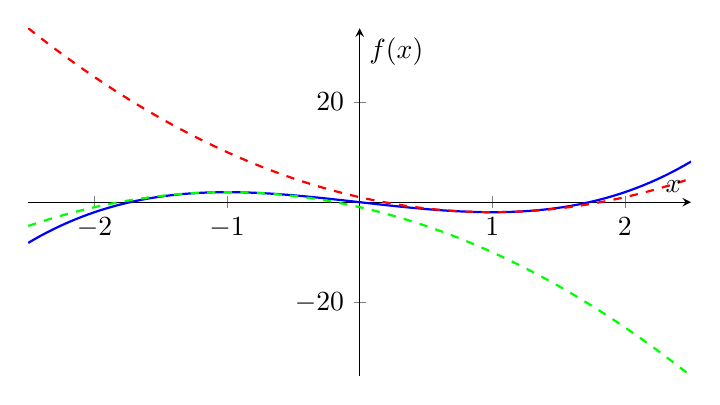
\begin{tikzpicture}
		\begin{axis}[
				axis lines = middle,
				xlabel = $x$,
				ylabel = $f(x)$,
				domain=-2.5:2.5,
				samples=100,
				legend pos=north west,
				legend cell align={left},
				width=10cm,
				height=6cm
			]
			% Plot the original function
			\addplot [blue, thick] {x^3 - 3*x};

			% Parabola approximation at x = 1
			\addplot [red, dashed, thick] {-2 + 3*(x-1)^2};

			% Parabola approximation at x = -1
			\addplot [green, dashed, thick] {2 - 3*(x+1)^2};

		\end{axis}
	\end{tikzpicture}
\end{figure}


(泰勒展开取极值,考试)
\subsubsection{量子力学}
在薛定谔方程当中,最为重要的是找出相应的哈密顿量$\cal H$,这也就意味着,找出哈密顿量中的的势能项,我们将势能写为这样的形式
\[
	V(x)=\frac{1}{2}m\omega^2x^2
\]
写出我们的薛定谔方程
\[
	-\frac{\hbar^2}{2m}\frac{\partial^2\psi}{\partial x^2}+\frac{1}{2}m\omega^2x^2\psi=E\psi
\]

\paragraph{偏微分方程解法}
首先,我们将要求$y=kx$,于是,我们便可以的得到$k\frac{\partial}{\partial y}=\frac{\partial}{\partial x}$

将其平方一下得到
\[
	\frac{\partial^2}{\partial y^2}=\frac{\partial^2}{\partial x^2}
\]

代入到薛定谔方程当中
\[
	\frac{\hbar^2}{2m}\frac{\partial^2}{\partial y^2}+\frac{1}{2}\frac{m\omega^2}{k^2}y^2\psi=E\psi
\]

再做一部小小的化简\\

再令$k=\sqrt{\dfrac{2mE}{\hbar^2}\omega}$

于是,我们便可以的得到
\[\frac{\partial^2}{\partial y^2} \psi -y^2\psi+K\psi=0\]

令$\psi(y)=\phi(y)H(y)$
要求,$\displaystyle \dfrac{\partial^2}{\partial y^2}\phi(y)=y^2\phi(y)$
可以让
\[\phi(y)=Ae^{\pm \frac{y^2}{2}}\]

考虑到波函数不可能是一个发散的函数,因此
\[\phi(y)=Ae^{- \frac{y^2}{2}}\]

下面我们来进行一下化简
\begin{align*}
	\psi^{\prime}       & =H^\prime\phi+H\phi^\prime                    \\
	\psi^{\prime\prime} & =H^\prime\prime\phi+2H^{'}\phi^{'}+H\phi^{''}
\end{align*}

同时,我们还有
\begin{align*}
	\phi^{'}  & =-y\phi   \\
	\phi^{''} & =-y^2\phi
\end{align*}

将其带入到之前已经化简完成的方程$\displaystyle \frac{\partial^2}{\partial y^2} \psi -y^2\psi+K\psi=0$可以得到
\[H^{''}\phi+2H^{'}\phi^{'}+(K+1)H\phi=0\]

对其进一步的化简
\[\left[H^{''}+2yH^{'}+(K+1)H\phi=0\right]\]

这也就意味着
\[H^{''}+2yH^{'}+(K+1)H=0\]

对函数$H$进行泰勒展开
\[
	H(y)=\sum_{n=0}^{\infty}a_ny^n
\]

那么,对$H(y)$进行求导
\[
	H^{'}(y)=\sum_{n=0}^{\infty}na_{n+1}y^{n}
\]

再对其求一次导
\[
	H^{''}(y)=\sum_{n=0}^{\infty}(n+2)(n+1)a_{n+2}y^{n}
\]

将其带入,可以对中得到关于$a_n$的递推关系式
\[a_{n+2}=\frac{2n+1-K}{(n+2)(n+1)}a_n\]

接下来我们来预测一下这个多项式$H(y)$的趋势

可以得出
\[H(y)\approx e^{y^2}\]

这将会导致波函数的发散,因此,我们要求$n$应当有一个最大值,并且使得接下来的$a_{n+2}=0$,
\[2n+1-K=0\]

所以,得到了这样的关系
\begin{align*}
	K=2n+1=\frac{2E}{\hbar\omega}
\end{align*}

于是得到了能量的表达式
\[
	E=\hbar\omega(n+\frac{1}{2})
\]

\paragraph{代数解法}\

首先写出我们的薛定谔方程
\begin{align*}
	-\frac{\hbar^2}{2m}\frac{\partial^2\psi}{\partial x^2}+\frac{1}{2}m\omega^2x^2\psi=E\psi
\end{align*}




先稍微做一些分离
\begin{align*}
	-\frac{\hbar^2}{2m}\frac{\partial^2\psi}{\partial x^2}+\frac{1}{2}m\omega^2x^2\psi & =\frac{1}{2m}\left[\left(\frac{\hbar}{i}\frac{\partial}{\partial x}\right)^2+(m\omega x)^2\right]\psi                        \\
	                                                                                   & =\frac{1}{2m}\left[\hat{p}^2+(m\omega x)^2\right]                                                                            \\
	                                                                                   & =\frac{1}{2m}(i\hat{p}+m\omega x)(-i\hat{p}+m\omega x)                                                                       \\
	                                                                                   & =\frac{1}{2m}\left(\hbar\frac{\partial}{\partial x}+m\omega x\right)\left(-\hbar\frac{\partial}{\partial x}+m\omega x\right)
\end{align*}

同时我们也定义了升降算符
\[ a_{\pm }\equiv \frac{1}{\sqrt{2\hbar m\omega}}(\mp ip +m\omega x)\]

通过计算,我们可以发现
\[a_{-}a_{+}=\mathcal{H}+\frac{1}{2}\hbar\omega\]
\[a_{+}a_{-}=\mathcal{H}-\frac{1}{2}\hbar\omega\]
\[a_{-}a_{+}-a_{+}a_{-}=\left[a_{-},a_{+}\right]=\hbar\omega\]

除此以外,当我们将哈密顿量$\mathcal{H}$作用在$(a_{-}\ket{\psi})$上时,我么可以发现一个阶梯式的变化
\begin{align*}
	\mathcal{H}\left(a_{-}\ket{\psi}\right) & =a_{-}(a_{+}a_{-}+\frac{1}{2}\hbar\omega)\ket{\psi}               \\
	                                        & =a_{-}\left(a_{-}a_{+}\frac{1}{2}\hbar\omega\right)\ket{\psi}     \\
	                                        & =a_{-}\left(\mathcal{H}-\frac{1}{2}\hbar\omega\right)\ket{\psi}   \\
	                                        & =(\mathcal{H}-\frac{1}{2}\hbar\omega)\left(a_{-}\ket{\psi}\right)
\end{align*}
而对于$(a_{+}\ket{\psi})$也是一样的效果,只不过是变成了加法,当然,这也是我们将这两个算符成为升降算符的主要原因。



\subsubsection{含时薛定谔方程简论}
在书写自由粒子的章节之前,我认为有必要去先简单的介绍一下含时薛定谔方程
\[
	i\hbar\frac{\partial}{\partial t}\Psi(\textbf{r},t)=H\Psi(\textbf{r},t)
\]

关于含时薛定谔方程的求解,传统方式都是关于位置与时间的分离变量,并且分离变量法能够很自然的给出含时薛定谔方程的特解,它有预测不含时可测量量的反直觉特性,很容易让我们困惑量子力学当中的时间去哪里了,而含时薛定谔方程的通解是特解的任意叠加,只有考虑到这种叠加,我们才可以观察到量子力学中观察到含时行为。




\subsection{自由粒子}
首先给出我们的定态薛定谔方程
\[
	-\frac{\hbar^2}{2m}\frac{\partial^2\psi}{\partial x^2}+V(x)\psi=E\psi
\]

很显然,由于是自由粒子,因此我们很容易的就可以知道它的势能应该是$0$

于是我们现在要求解的薛定谔方程为
\[
	-\frac{\hbar^2}{2m}\frac{\partial^2\psi}{\partial x^2}=E\psi
\]

对于这种方程,我们可以很轻松的得到它的解
\[\psi(x)=Ae^{ikx}+Be^{-ikx}\]

于是完整的含时波函数为
\[\psi(x,t)=Ae^{ikx-i\frac{E}{\hbar} t}+Be^{-ikx-i\frac{E}{\hbar} t}\]

能量$E$和$k$的关系有
\[
	k=\sqrt{\frac{2mE}{\hbar^2}}
\]

于是可以将含时波函数写为
\[
	\psi(x,t)=Ae^{ik(x+\frac{k\hbar}{2m}t)}+Be^{-ik(x-\frac{k\hbar}{2m}t)}
\]
对于这两部分它的前一项可以类比成一个向前运动的波,而后一项可以类比成一个反方向运动的波。

但是当我们对波函数进行归一化的时候出现了很大的问题
\[\psi_k(x,t)=Ae^{ik(x+\frac{k\hbar}{2m}t)}\]
\[\int_{-\infty}^{\infty}|\psi(x,t)|^2dx=\int_{-\infty}^{\infty}A^2\cdot\infty dx\]

也就是说$\psi_k$无法归一化,说明
\begin{enumerate}
	\item 对于自由粒子而言,分离变量解在物理上并不能够代表物理上可观测的量。
	\item 一个自由粒子不能存在一个定态。
	\item 不存在一个自由粒子具有确定能量这样的事情,关于能量守恒,我们也可以认为,是测到处于某个能量的概率不随着时间变化,而不是经典力学当中能量的数值是不变的。
\end{enumerate}

\paragraph{自由粒子的波包}\ \\

\begin{figure}[h!]
	\centering
	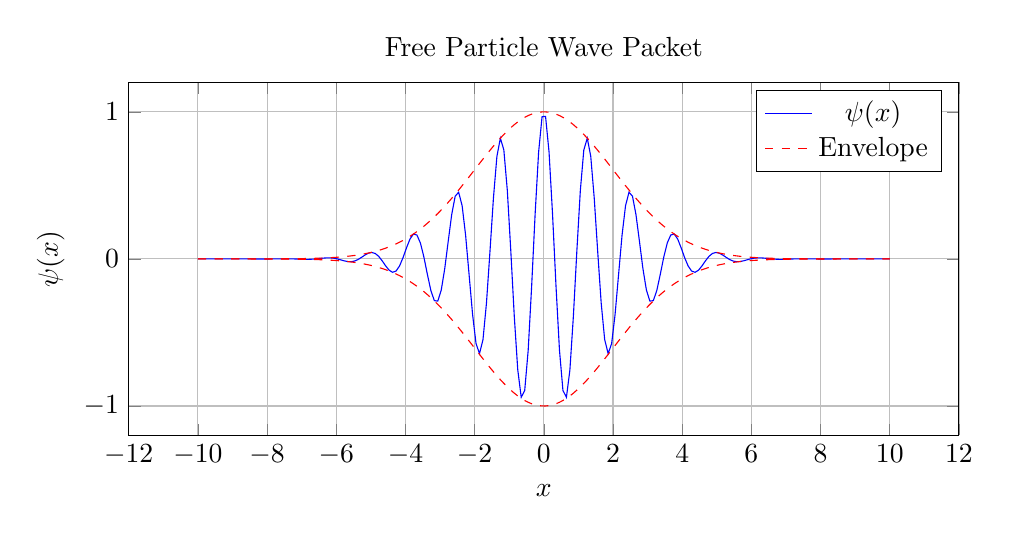
\begin{tikzpicture}
		\begin{axis}[
				xlabel = {$x$},
				ylabel = {$\psi(x)$},
				title = {Free Particle Wave Packet},
				grid = both,
				width = \textwidth,
				height = 0.5\textwidth
			]
			\addplot[
				domain=-10:10,
				samples=200,
				color=blue,
			]
			{exp(-0.5 * (x / 2)^2) * cos(deg(5 * x))};

			\addplot[
				domain=-10:10,
				samples=200,
				color=red,
				dashed
			]
			{exp(-0.5 * (x / 2)^2)};

			\addplot[
				domain=-10:10,
				samples=200,
				color=red,
				dashed
			]
			{-exp(-0.5 * (x / 2)^2)};

			\legend{$\psi(x)$, Envelope}
		\end{axis}
	\end{tikzpicture}
	\caption{Free Particle Wave Packet and Its Envelope}
	\label{fig:wave-packet}
\end{figure}





下面我们重新给出一维自由粒子的波函数形式:
\[\Psi(x,t)=Ae^{i(kx-\omega t)}\]

根据线性方程的可叠加性,这个平面波的所有线性组合均能够成为自由粒子波函数的解,因此,波动方程可以写为:
\[\Psi(x,t)=\frac{1}{\sqrt{2\pi}}\int g(k)e^{i\left[k\cdot x-\omega(k)t\right]}dk\]
对于初始时刻$t=0$,波函数为
\[\Psi(x,0)=\frac{1}{\sqrt{2\pi}}\int g(k)e^{i\left[k\cdot x-\omega(k)0\right]}dk=\frac{1}{\sqrt{2\pi}}\int g(k)e^{ikx}dk\]
可以看出$g(k)$其实是傅里叶变换的结果,因此,我们可以认为$g(k)$是一个谱函数,它描述了在空间上,不同频率的能量分布。


\paragraph{$|g(k)|$对波包的影响}\ \\


\begin{figure}[hbtp]
	\centering
	\begin{subfigure}[b]{0.9\textwidth}
		\centering
		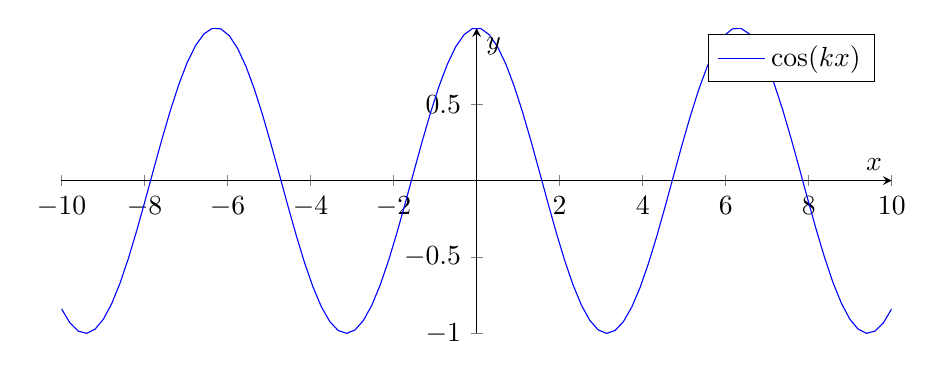
\begin{tikzpicture}
			\begin{axis}[
					axis lines = middle,
					xlabel = {$x$},
					ylabel = {$y$},
					width = \textwidth,
					height = 0.45\textwidth,
					domain = -10:10
				]
				\addplot[domain=-10:10,samples=100,blue] {cos(deg(x))};
				\addlegendentry{$\cos(kx)$}
			\end{axis}
		\end{tikzpicture}
		\caption{$\cos(kx)$}
		\label{fig:coskx}
	\end{subfigure}

	\begin{subfigure}[b]{0.9\textwidth}
		\centering
		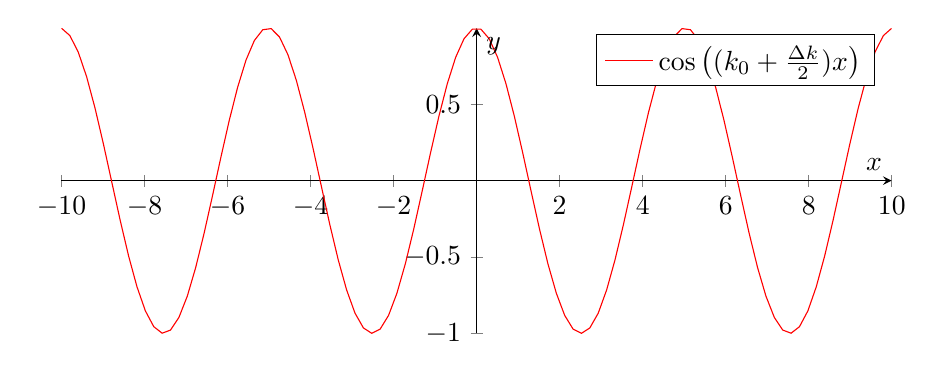
\begin{tikzpicture}
			\begin{axis}[
					axis lines = middle,
					xlabel = {$x$},
					ylabel = {$y$},
					width = \textwidth,
					height = 0.45\textwidth,
					domain = -10:10
				]
				\addplot[domain=-10:10,samples=100,red] {cos(deg((1+0.5/2)*x))};
				\addlegendentry{$\cos\left((k_0 + \frac{\Delta k}{2})x\right)$}
			\end{axis}
		\end{tikzpicture}
		\caption{$\cos\left((k_0 + \frac{\Delta k}{2})x\right)$}
		\label{fig:coskplusdx}
	\end{subfigure}

	\begin{subfigure}[b]{0.9\textwidth}
		\centering
		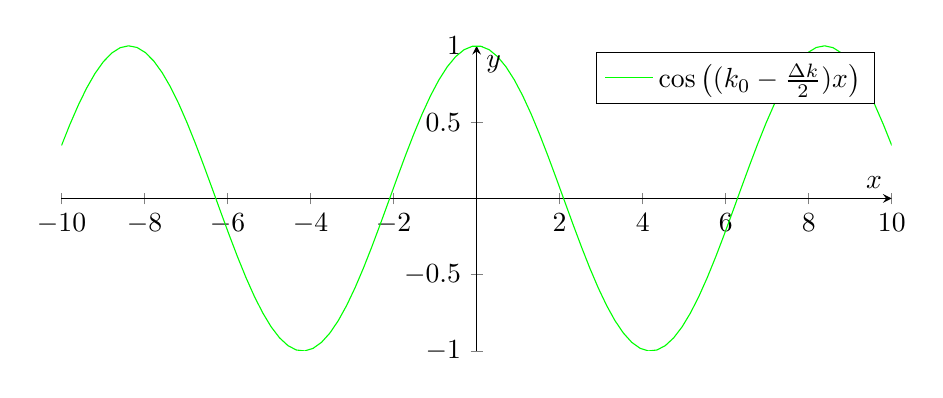
\begin{tikzpicture}
			\begin{axis}[
					axis lines = middle,
					xlabel = {$x$},
					ylabel = {$y$},
					width = \textwidth,
					height = 0.45\textwidth,
					domain = -10:10
				]
				\addplot[domain=-10:10,samples=100,green] {cos(deg((1-0.5/2)*x))};
				\addlegendentry{$\cos\left((k_0 - \frac{\Delta k}{2})x\right)$}
			\end{axis}
		\end{tikzpicture}
		\caption{$\cos\left((k_0 - \frac{\Delta k}{2})x\right)$}
		\label{fig:coskminusdx}
	\end{subfigure}

	\begin{subfigure}[b]{0.9\textwidth}
		\centering
		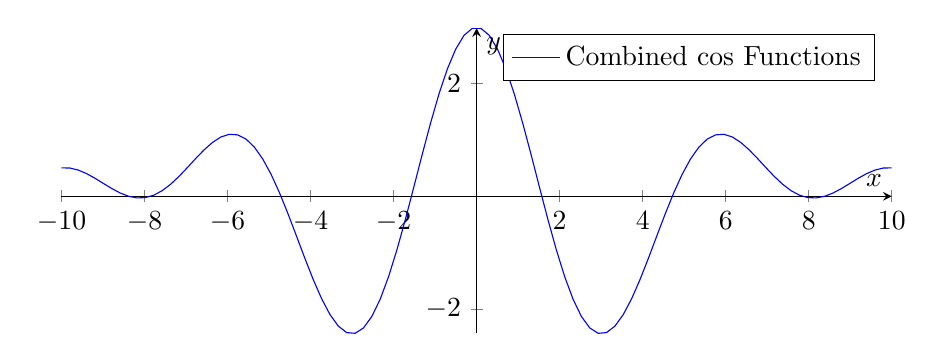
\begin{tikzpicture}
			\begin{axis}[
					axis lines = middle,
					xlabel = {$x$},
					ylabel = {$y$},
					width = \textwidth,
					height = 0.45\textwidth,
					domain = -10:10
				]
				\addplot[domain=-10:10,samples=100,blue] {cos(deg(x)) + cos(deg((1+0.5/2)*x)) + cos(deg((1-0.5/2)*x))};
				\addlegendentry{Combined $\cos$ Functions}
			\end{axis}
		\end{tikzpicture}
		\caption{Combined Cosine Function}
		\label{fig:combined}
	\end{subfigure}

	\caption{Plots of $\cos(kx)$, $\cos\left((k_0 + \frac{\Delta k}{2})x\right)$, $\cos\left((k_0 - \frac{\Delta k}{2})x\right)$ and their combination}
\end{figure}




为了研究对波包的影响,我们首先不考虑无穷个波包叠加的形式,而是先只考虑部分波包的叠加,首先尝试研究仅三个波函数叠加的情况,我们选取波矢为$\displaystyle k_0,k_0+\frac{\Delta k}{2},k_0-\frac{\Delta k}{2}$,他们的振幅分别为$1,\frac{1}{2},\frac{1}{2}$进行叠加:
\begin{align*}
	\Psi(x,t) & =\frac{g(k_0)}{\sqrt{2\pi}}\left[e^{ik_0x}+\frac{1}{2}e^{i(k_0-\frac{\Delta k}{2}+\frac{1}{2}e^{i(k_0+\frac{\Delta k}{2})})}\right] \\
	          & =\frac{g(k_0)}{\sqrt{2\pi}}e^{ik_0x}\left[1+\cos(\frac{\Delta k}{2})\right]
\end{align*}

当他们的相位差达到$\pi$时,$|\Psi|=0$,而此时的$\cos(\frac{\Delta k\Delta x}{2})=-1$,因此可以求得$\Delta k\Delta x=4\pi$

这样的等式向我们表明,当$|g(k)|$的$\Delta k$越小,也就是峰越窄的时候,波包的实际宽度便越大,反之亦然。







\begin{figure}[hbtp]
	\centering
	\begin{tikzpicture}
		\begin{axis}[
				xlabel = {$k$},
				ylabel = {$|\Psi(k)|$},
				title = {Frequency Domain of Free Particle Wave Function},
				grid = both,
				width = 0.4\textwidth,
				height = 0.2\textheight
			]
			\addplot[
				domain=-10:10,
				samples=200,
				color=blue,
			]
			{sqrt(pi) * (exp(-((x-5)^2)/4) + exp(-((x+5)^2)/4))};
		\end{axis}
	\end{tikzpicture}
	\caption{Frequency Domain of Free Particle Wave Function}
	\label{fig:frequency-domain}
\end{figure}




\paragraph{$g(k)$的辐角}\ \\
事实上,在上面的讨论当中,我们讨论的是$|g(k)|$,但是却没有讨论到复值,因此,我们将$g(k)$在$k$处的辐角取为$\alpha(k)$,故我们设$g(k)=|g(k)|e^{i\alpha(k)}$.

此时我们可以将波函数写作:
\[
	\Psi(x,t)=\frac{1}{\sqrt{2\pi}}\int_{-\infty}^{\infty}g(k)e^{ikx}dk
\]

当最大值附近的波能够最大程度的叠加时就能够出现最大值,也就是说,$k_0$附近的波有较大的相位差,则在整个范围内的上下振荡会很大,因此正负很快就会相互抵消,积分值趋近于$0$。

因此,假设在积分达到最大值时$x=x_0$,对$k$的变化率为$0$时,
\[
	\frac{d\left[kx_0+\alpha(k)\right]}{dk}=0
\]

可以推出:
\[
	x_0=\left.\frac{d\alpha(k)}{dk}\right|_{x=x_0}
\]

此时,我们假定在区间$\left[k_0-\frac{\Delta k}{2},k_0+\frac{\Delta k}{2}\right]$内,$\alpha(k)$的变化是足够光滑的,并且当$\Delta k$足够小时,$\alpha(k)$可以在$k_0$附近泰勒展开,经过尝试,在这里我们取到两项:
\begin{align}
	\alpha(k) & =\alpha(k_0)+\left(k-k_0\right)\left.\frac{d\alpha(k)}{dk}\right|_{k=k_0} \\
	          & =\alpha(k_0)-(k-k_0)x_0
\end{align}

将其代入到
\[\Psi(x,0)=\frac{1}{\sqrt{2\pi}}\int g(k)e^{i\left[kx\right]dk}\]

我们可以得到
\begin{align*}
	\Psi(x,0) & =\frac{1}{\sqrt{2\pi}}e^{\alpha(k_0)}\int g(k)e^{i\left[kx-(k-k_0)x_0\right]dk}       \\
	          & =\frac{1}{\sqrt{2\pi}}e^{\alpha(k_0)-k_0x}\int g(k)e^{i\left[(k-k_0)(x-x_0)\right]dk}
\end{align*}

当$x$逐渐远离$x_0$时,$|\Psi|$也将逐渐减小,当$x$增大到$e^{i\left[(k-k_0)(x-x_0)\right]}$约在$\Delta k$区间内振荡一次时,减小变得明显。此时$\Delta k(x-x_0)\backsimeq 1$.如果这时,我们让波包的宽度大致为$\Delta x\geqslant x-x_0$,则有:
\[
	\Delta k\Delta x\geqslant  \thickapprox 1
\]













\begin{figure}[h]
	\centering
	\begin{subfigure}[b]{0.45\textwidth}
		\centering
		\begin{tikzpicture}
			\begin{axis}[
					xlabel={$k$},
					ylabel={$\text{Re} \{ g(k) e^{i(k - k_0)(x - x_0)} \}$},
					axis lines=middle,
					width=\textwidth,
					height=0.25\textheight,
					xtick=\empty,
					ytick=\empty,
					ymin=-1.5, ymax=1.5,
					xmin=-3, xmax=3,
					domain=-3:3,
					samples=100
				]
				\addplot [black, thick, dashed] {exp(-x^2)};
				\addplot [black, thick] {exp(-x^2) * cos(deg(10*x))};
				\node at (axis cs:0.5,-1.2) {$k_0$};
				\node at (axis cs:2,-0.5) {$|x - x_0| > \frac{1}{\Delta k}$};
			\end{axis}
		\end{tikzpicture}
		\caption{(a)}
	\end{subfigure}
	\hfill
	\begin{subfigure}[b]{0.45\textwidth}
		\centering
		\begin{tikzpicture}
			\begin{axis}[
					xlabel={$k$},
					ylabel={$\text{Re} \{ g(k) e^{i(k - k_0)(x - x_0)} \}$},
					axis lines=middle,
					width=\textwidth,
					height=0.25\textheight,
					xtick=\empty,
					ytick=\empty,
					ymin=-1.5, ymax=1.5,
					xmin=-3, xmax=3,
					domain=-3:3,
					samples=100
				]
				\addplot [black, thick, dashed] {exp(-x^2)};
				\addplot [black, thick] {exp(-x^2) * cos(deg(2*x))};
				\node at (axis cs:0.5,-1.2) {$k_0$};
				\node at (axis cs:2,-0.5) {$|x - x_0| < \frac{1}{\Delta k}$};
			\end{axis}
		\end{tikzpicture}
		\caption{(b)}
	\end{subfigure}
	\caption{(a) $|x - x_0| > \frac{1}{\Delta k}$ and (b) $|x - x_0| < \frac{1}{\Delta k}$}
\end{figure}




\paragraph{群速度与相速度}\ \\

首先讲一下相速度,顾名思义,相速度应该就是所谓的相位的变化速度,因此,我们可以将其写作为
\[
	v_{phase}=\frac{\omega}{k}
\]

对于群速度,我们可以认为是整个波包的运动速度,就好像是一群粒子一样,因此我们将其定义为
\[
	v_{group}=\Da{\omega}{k}
\]

从这边可以看出,如果在运动的时候如果没有产生所说的波包,那么它的群速度和相速度应当是一致的。

在自由粒子波包的情况当中,我们的$\omega = \frac{\hbar k^2}{2m}$,因此可以算出
\begin{align*}
	v_{group} & =2\frac{\hbar k}{2m} \\
	v_{phaes} & =\frac{\hbar k}{2m}
\end{align*}
刚刚好群速度是相速度的$2$倍。

\subsection{狄拉克函数势}

考虑到该形式下的势能为
\[V(x)=-\alpha\delta(x)\]

\begin{figure}[hbtp]
	\centering
	\begin{tikzpicture}
		\draw[->] (-2,0) -- (2,0) node[right] {$x$};
		\draw[->] (0,-1.5) -- (0,1.5) node[above] {$V(x)$};
		\draw[-, thick] (-2,0) -- (0,0);
		\draw[->, ultra thick] (0,0) -- (0,-1);
		\draw[-, thick] (0,0) -- (2,0);
		\node[below] at (0,-1) {$-\lambda\delta(x)$};
	\end{tikzpicture}
\end{figure}

首先写出薛定谔方程
\[
	i\hbar\frac{\partial}{\partial t}\Psi(x,t)=-\frac{\hbar^2}{2m}\frac{\partial^2}{\partial x^2}\Psi(x,t)+\alpha\delta(x)\Psi(x,t)
\]
从$\delta(x)$函数的图我们可以定义出波函数的两个态
\subsubsection{束缚态与散射态}
关于束缚态,我们有很容易的区分方式,只需要对势能进行判断即可:

\begin{enumerate}
	\item[$\cdot$] 束缚态: $V < 0$
	\item[$\cdot$] 散射态: $V > 0$
\end{enumerate}


\subsubsection{求解}

我们的任务首先是对$x\neq 0$部分的求解,在这部分,势能$V(x)$为$0$,因此薛定谔方程可以直接写为
\[
	E\psi(x)=-\frac{\hbar^2}{2m}\frac{\partial^2}{\partial x^2}\psi(x)
\]

通过移项我们最后可以得到波动方程的形式
\[
	\frac{d^2\psi}{dx^2}=-\frac{2mE}{\hbar^2}\psi=\kappa^2\psi
\]
其中$\displaystyle\kappa=\sqrt{-\dfrac{2mE}{\hbar^2}}$

通过求解我们可以得到波动方程的解
\[
	\psi(x)=Ae^{-i\kappa x}+Be^{i\kappa x},\quad x<0
\]
\[\psi(x)=Fe^{-i\kappa x}+Ge^{i\kappa x},\quad x>0\]

首先当$x\to-\infty$时,波函数的第一项将会趋近于无穷,因此我们必须让$A=0$:
\[
	\psi(x)=Be^{i\kappa x},\quad x<0
\]

而在$x\to\infty$时,波函数的第二项将会趋近于无穷,因此我们必须让$G=0$:
\[
	\psi(x)=Fe^{i\kappa x},\quad x>0
\]




波函数求解的边界条件
\begin{enumerate}
	\item 波函数$\psi(x)$是连续的
	\item $\dfrac{\partial\psi}{\partial x}$除了势是无穷大的点外是连续的
\end{enumerate}

在这道题的情况当中,我们可以利用第一个边界条件,这个条件告诉我们
\[F=B\]

因此我们的波函数可以写为
\begin{equation*}
	\psi(x)=
	\begin{cases}
		Be^{i\kappa x},\quad x<0 \\
		Be^{-i\kappa x},\quad x>0
	\end{cases}
\end{equation*}


但是由于我们的$\delta$函数势使得$\frac{d\psi}{dx}$在$x=0$处是不连续的,这将导致我们的第二个边界条件使用不起来,现在我们来看一下$\delta$函数的作用,作为一个副产物,我们讲明白为什么通常情况下$\frac{d\psi}{dx}$是连续的。

首先我们绕过那个不连续点$x=0$,在区间$[-\varepsilon,\varepsilon]$上对薛定谔方程进行积分
\[
	\int_{-\varepsilon}^{\varepsilon}E\psi(x)dx=\int_{-\varepsilon}^{\varepsilon}-\frac{\hbar^2}{2m}\frac{\partial^2}{\partial x^2}\psi(x)dx+\int_{-\varepsilon}^{\varepsilon}V(x)\psi(x)dx
\]

取当$\varepsilon\to 0$时的极限,将这个积分计算一下可以得到
\[
	\lim_{\varepsilon\to0}\left(\left.\frac{d\psi}{dx}\right|_{\varepsilon}-\left.\frac{d\psi}{dx}\right|_{-\varepsilon}\right)=\frac{2m}{\hbar^2}\int_{-\varepsilon}^{\varepsilon}V(x)\psi(x)dx
\]

这样的话就无需$\dfrac{d\psi}{dx}$在$x=0$处是连续的了,我们只要分别去找到它的左导数和右导数就可以得出结果
\begin{align*}
	-2B\kappa & =-\frac{2m}{\hbar^2}\alpha\psi(0) \\
	\kappa    & =\frac{\alpha m}{\hbar^2}
\end{align*}

但是非常遗憾的是,这个条件最终求解下来,并没有能够求得$B$,此时使用我们最后的手段,归一化条件




\subsubsection{讨论$E>0$}

此时,我们将$k\equiv \frac{\sqrt{2mE}}{\hbar}$

由此,可以将薛定谔方程写为
\[
	\frac{d^2\psi}{dx^2}=-\frac{2mE}{\hbar^2}\psi=-k^2\psi
\]

很明显,我们可以得出平面波解
\begin{center}
	\begin{enumerate}
		\item $x<0$,$\psi_1(x)=Ae^{ikx}+Be^{-ikx}$
		\item $x>0,\psi_2(x)=Fe^{ikx}+Ge^{-ikx}$
	\end{enumerate}
\end{center}


在这里,我们知道$A,F$是一个向前传播的波,而$B,G$是一个向后传播的波。

首先任然是利用连续条件来求解四个未定系数
\[\psi_1(0)=\psi_2(0)\]

很自然的便可以得到
\[A+B=F+G\]

接下来,任然是对薛定谔方程进行积分,可以得到
\[
	\lim_{\varepsilon\to0}\left(\left.\frac{d\psi_1}{dx}\right|_{\varepsilon}-\left.\frac{d\psi_2}{dx}\right|_{-\varepsilon}\right)=\frac{2m}{\hbar^2}\int_{0}^{\varepsilon}V(x)\psi_1(x)dx-\frac{2m}{\hbar^2}\int_{0}^{\varepsilon}V(x)\psi_2(x)dx
\]

化简可以得到
\[ik(F-G-A+B)=-\frac{2m\alpha}{\hbar^2}(A+B)=-\frac{2m\alpha}{\hbar^2}(F+G)\]

很显然,我们现有的条件所得到的方程在数学上是没有办法求解的,可是在物理上,很明显,如果是一个波从左向右传播,那么可以有反射波也可以有透射波,可是这样的话,我们可以知道并没有$G$所能够表征的波,因此,$G=0$


\paragraph{透射率与反射率}

我们下面来定义一下透射率和反射率
\begin{enumerate}
	\item 反射率\[R=\frac{J_{ref}}{J_{in}}\]
	\item 透射率\[T=\frac{J_{trans}}{J_{in}}\]
\end{enumerate}

几率流密度$J$
\[
	J(x)=-\frac{i\hbar}{2m}\left[\psi^{*}\frac{\partial\psi}{\partial x}-\frac{\partial \psi^{*}}{\partial x}\psi\right]
\]

根据这个定义,我们可以去计算入射波、反射波、透射波的几率流密度
\begin{center}
	\begin{enumerate}
		\item 入射波\[J_{in}=\frac{\hbar k}{m}\left|A\right|^2\]
		\item 反射波\[J_{ref}=\frac{\hbar k}{m}\left|B\right|^2\]
		\item 透射波\[J_{trans}=\frac{\hbar k}{m}\left|F\right|^2\]
	\end{enumerate}
\end{center}

于是可以计算出透射率与反射率
\[
	R=\frac{J_{ref}}{J_{in}}=\frac{\beta^2}{1+\beta^2}
\]
\[
	T=\frac{J_{trans}}{J_{in}}=\frac{1}{1+\beta^2}
\]

其中
\[\beta=\frac{m\alpha}{k\hbar^2}\]

进一步化简,可以得到
\[
	R=\frac{1}{1+\frac{2\hbar^2E}{m\alpha^2}}
\]

\[
	T=\frac{1}{1+\frac{m\alpha^2}{2\hbar^2E}}
\]

从这个结论可以发现
\begin{enumerate}
	\item 当$E$足够大的时候,透射率几乎为$1$,也就是全都过去了
	\item 当质量$m$足够大的时候,几乎完全被反射(?)
	\item 当$\alpha$足够大的时候,也几乎同时被反射(?)
\end{enumerate}



\subsection{有限方势垒}

首先给出势能的函数
\begin{align*}
	V(x)=
	\begin{cases}
		V, & \quad0<x<L            \\
		0, & \quad\text{elsewhere}
	\end{cases}
\end{align*}
首先是对于势能为$0$部分的薛定谔方程的求解,这在我们之前已经遇到了好几次



我们的重点在于求解出势能不为$0$的部分,也就是在$0<x<L$的区间内



\section{三维薛定谔方程}

首先还是写出我们的三维薛定谔方程
\[
	\left[-\frac{\hbar^2}{2m}\nabla^2+V(\textbf{r})\right]\psi=i\hbar\frac{\partial\psi}{\partial t}
\]

其中,哈密顿量$\displaystyle\mathcal{H}=-\frac{\hbar^2}{2m}\nabla^2-V(\textbf{r})$,波函数为$\psi=\psi(\textbf{r},t)\\$

与此同时,也有一些东西要改,首先是归一化条件
\[
	\int_{-\infty}^{\infty}\psi^*(\textbf{r},t)\psi(\textbf{r},t)d^3r=\int_{-\infty}^{+\infty}\psi^*(\textbf{r},t)\psi(\textbf{r},t)d^3r=1
\]
\subsection{数学准备————球坐标系,$\nabla$算符}
为了能够充分利用到我们的三维空间,但是笛卡尔坐标系$(x,y,z)$又会很复杂,因此,我们转化到球坐标系进行计算,下面我们将复习一下球坐标系$(r,\theta,\phi)$
首先给出坐标变换的关系,以方便我们将薛定谔方程转化到球坐标系当中
\[
	\begin{cases}
		x=r\sin\theta\cos\phi                                                        \\
		y=r\sin\theta\sin\phi                                                        \\
		z=r\cos\theta                                                                \\
		r=\sqrt{x^2+y^2+z^2}                                                         \\
		\theta=\arccos\left(\frac{z}{r}\right)=\arctan\left(\frac{x^2+y^2}{z}\right) \\
		\phi=\atan2(y,x)=
		\begin{cases}
			\arctan\left(\frac{y}{x}\right),     & \quad x>0     \\
			\arctan\left(\frac{y}{x}\right)+\pi, & \quad x<0,y>0 \\
			\arctan\left(\frac{y}{x}\right)-\pi, & \quad x<0,y<0 \\
			\frac{\pi}{2},                       & \quad x=0,y>0 \\
			-\frac{\pi}{2},                      & \quad x=0,y<0 \\
			undefined,                           & \quad x=y=0
		\end{cases}
	\end{cases}
\]

为了进行坐标转换,我们定义一个scale factor $h_i$,使得
\begin{equation*}
	h_i=\sqrt{\sum_{k}\left(\frac{\partial x_k}{\partial q_i}\right)^2}
\end{equation*}

因此可以得到
\[
	\begin{cases}
		h_r      & =1           \\
		h_\theta & =r           \\
		h_\phi   & =r\sin\theta
	\end{cases}
\]

\subsubsection{$\nabla$算符与它的运算}
\begin{enumerate}
	\item 梯度(gradient)
	      \begin{equation*}
		      \nabla S =\left(\sum_{i}\hat{e_i}\frac{1}{h_i}\Da{~}{q_i}\right)=\left(\hat{e_{r}}\Da{~}{r}+\hat{e_\theta}\frac{1}{r}\Da{~}{\theta}+\hat{e_\psi\frac{1}{r\sin\theta}\Da{~}{\phi}}\right)
	      \end{equation*}
	\item 散度(divergence)
	      \[
		      \nabla\cdot \vec{S}=\frac{1}{h_1h_2h_3}\sum_{i}\frac{1}{h_i}\Da{~}{q_i}(h_jh_kS_i)
	      \]
	\item 拉普拉斯算符(Laplacian)
	      \[
		      \nabla^2 S=\nabla\cdot\nabla S=\frac{1}{h_1h_2h_3}\sum_{i}\frac{1}{h_i}\Da{~}{q_i}\left(\frac{h_jh_k}{h_i}\Da{~}{q_i}S\right)
	      \]
	\item 旋度(curl)
	      \[
		      \nabla\times\vec{S}=\frac{1}{h_1h_2h_3}\vmthree{h_1\hat{e_1}}{h_2\hat{e_2}}{h_3\hat{e_3}}{\displaystyle\Da{~}{r}}{\displaystyle\Da{~}{\theta}}{\displaystyle\Da{~}{\phi}}{h_1S_1}{h_2S_2}{h_3S_3}
	      \]
\end{enumerate}

这其中对于我们接下来求解三维球坐标薛定谔方程最为重要的还是拉普拉斯算子,经过化简,我么可以得到
\[
	\nabla^2 S=\frac{1}{r^2}\frac{\partial}{\partial r}\left(r^2\frac{\partial}{\partial r}S\right)+\frac{1}{r^2\sin\theta}\frac{\partial}{\partial\theta}\left(\sin\theta\frac{\partial}{\partial\theta}S\right)+\frac{1}{r^2\sin^2\theta}\frac{\partial^2}{\partial\phi^2}S
\]

\subsection{三维球坐标系的定态薛定谔方程}
首先将其写出
\[
	\left[-\frac{\hbar^2}{2m}\left(\frac{1}{r^2}\frac{\partial}{\partial r}\left(r^2\frac{\partial}{\partial r}\right)+\frac{1}{r^2\sin\theta}\frac{\partial}{\partial\theta}\left(\sin\theta\frac{\partial}{\partial\theta}\right)+\frac{1}{r^2\sin^2\theta}\frac{\partial^2}{\partial\phi^2}\right)+V(\textbf{r})\right]\psi=E\psi(r,\theta,\phi)
\]

老套路,分离变量
\[
	\psi(r,\theta,\phi)=R(r)Y(\theta,\phi)
\]

还是一样,代入到方程里面
\[
	\left[-\frac{\hbar^2}{2m}\left(\frac{1}{r^2}\frac{\partial}{\partial r}\left(r^2\frac{\partial}{\partial r}\right)+\frac{1}{r^2\sin\theta}\frac{\partial}{\partial\theta}\left(\sin\theta\frac{\partial}{\partial\theta}\right)+\frac{1}{r^2\sin^2\theta}\frac{\partial^2}{\partial\phi^2}\right)+V(\textbf{r})\right]R(r)Y(\theta,\phi)=ER(r)Y(\theta,\phi)
\]

等式两边同时除以$R(r)Y(\theta,\phi)$,可以得到
\begin{equation*}
	\frac{1}{R}\D{~}{r}\left(r^2\D{R}{r}\right)-\frac{2mr^2}{\hbar^2}\left[V(r)-E\right]+\frac{1}{Y}\frac{1}{\sin{\theta}}\Da{~}{\theta}\left(\sin{\theta}\Da{Y}{\theta}\right)+\frac{1}{\sin{\theta}^2}\frac{\partial^2 Y}{\partial \phi^2}=0
\end{equation*}

可以看出,这两个部分分别有不同的自变量进行控制,因此加号的前面一部分应该是等于一个常数,为了使得等式仍然为$0$,后一部分等于这个常数的相反数,我们人为的定义这个常数为$l(l+1)$(仅仅为了后面的计算方便),那么有
\begin{align*}
	\frac{1}{R}\D{~}{r}\left(r^2\D{R}{r}\right)-\frac{2mr^2}{\hbar^2}\left[V(r)-E\right]                                                                & =l(l+1)  \\
	\frac{1}{Y}\frac{1}{\sin{\theta}}\Da{~}{\theta}\left(\sin{\theta}\Da{Y}{\theta}\right)+\frac{1}{\sin{\theta}^2}\frac{\partial^2 Y}{\partial \phi^2} & =-l(l+1)
\end{align*}




\subsubsection{角动量方程}
首先给出角动量方程
\begin{align*}
	\frac{1}{Y}\frac{1}{\sin{\theta}}\Da{~}{\theta}\left(\sin{\theta}\Da{Y}{\theta}\right)+\frac{1}{\sin{\theta}^2}\frac{\partial^2 Y}{\partial \phi^2} & =-l(l+1)
\end{align*}

进一步的我们可以将$Y(\theta,\phi)=\Theta(\theta)\Phi(\phi)$进行变换,得到
\begin{align*}
	\left\{\frac{1}{\Theta}\left[\sin{\theta}\D{~}{\theta}\left(\sin{\theta}\D{~}{\theta}\Theta\right)\right]+l(l+1)\sin^2{\theta}\right\}+\frac{1}{\Phi}\frac{d^2}{d\phi^2}\Phi & =0
\end{align*}


很显然,这两个部分仍然是等于一个常数$m^2$,因此我们可以有
\begin{align*}
	\left\{\frac{1}{\Theta}\left[\sin{\theta}\D{~}{\theta}\left(\sin{\theta}\D{~}{\theta}\Theta\right)\right]+l(l+1)\sin^2{\theta}\right\} & =m^2      \\
	\frac{d^2}{d\phi^2}\Phi                                                                                                                & =-m^2\Phi
\end{align*}

一眼便可以看见一个我们非常熟悉的方程
\begin{align*}
	\frac{d^2}{d\phi^2}\Phi & =-m^2\Phi
\end{align*}

求解可得
\begin{align*}
	\Phi & =Ae^{im\phi}+Be^{-im\phi}
\end{align*}

假设我们的$m<0$

那么将会有
\begin{align*}
	\Phi & =Ae^{im\phi}
\end{align*}

此时我们有一个自然的边界条件
\begin{align*}
	\Phi(\theta)=\Phi(\theta+2\pi)
\end{align*}

于是得到$m$的取值为
\begin{align*}
	m=0,\pm 1,\pm 2,\cdots
\end{align*}

对于另外一个方程
\begin{equation*}
	\left\{\frac{1}{\Theta}\left[\sin{\theta}\D{~}{\theta}\left(\sin{\theta}\D{~}{\theta}\Theta\right)\right]+l(l+1)\sin^2{\theta}\right\}=m^2
\end{equation*}

这个方程的求解非常复杂,它的解是:
\begin{equation*}
	\Theta=AP_l^m(\cos{\theta})=(1-\cos^2{\theta})^{\frac{|m|}{2}}\left(\frac{d}{dx}\right)^{|m|}P_l(\cos{\theta})
\end{equation*}

接下来我们在利用一下归一化条件,
\begin{align*}
	\int|\psi|^2r^2\sin{\theta}drd\theta d\phi            & =1 \\
	\int|R|^2r^2dr\cdot\int|Y|^2\sin{\theta}d\theta d\phi & =1
\end{align*}

最终,我们归一化的角波函数我们将其称为角波函数$Y_l^m(\theta,\phi)$,表达式为
\begin{equation*}
	Y_l^m(\theta,\phi)=\varepsilon\sqrt{\frac{(2l+1)(l-|m|)!}{4\pi(l+|m|)!}}e^{im\phi}P_l^m(\cos{\theta})
\end{equation*}

\subsubsection{径向方程}
首先给出径向方程
\begin{align*}
	\frac{1}{R}\D{~}{r}\left(r^2\D{R}{r}\right)-\frac{2mr^2}{\hbar^2}\left[V(r)-E\right] & =l(l+1)
\end{align*}

为了求解的方便,我们人为定义$u(r)\equiv rR(r)$
于是,我们可以将方程写成
\begin{align*}
	-\frac{\hbar^2}{2m}\frac{d^2u}{dr^2}+\left[V(u)+\frac{\hbar^2}{2m}\frac{l(l+1)}{r^2}-E\right]u(r) & =0
\end{align*}

很显然,想要求解这样的方程我们需要知道势能$V(r)$,让我们直接来求解氢原子的波函数,因为它具有比较简单的势场。

说实话,接下来的求解方法和之前在求解一维简谐振子的方法可以说是一模一样,读者可以仿照自行进行求解,练练手,最后我不要脸的给出径向波函数。
\begin{align*}
	R_{nl}(r) & =\frac{1}{r}\rho^{l+1}e^{-\rho}v(\rho)            \\
	\rho      & =\frac{r}{an}                                     \\
	a         & =\frac{4\pi\varepsilon_0\hbar^2}{me^2}            \\
	v(\rho)   & =c_0\sum_{j=0}\frac{2^j}{j!}\rho^{j}=c_0e^{2\rho} \\
	c_{j+1}   & =\frac{2(j+l+1-n)}{(j+1)(j+2l+2)}c_{j}
\end{align*}

但是在求解过程中有些东西还是不太放心,放在这里说一下
\begin{enumerate}
	\item 求解过程中,我们会发现$v(\rho)=c_0\sum_{j=0}\frac{2^j}{j!}\rho^{j}=c_0e^{2\rho}$,这也就意味着$u(\rho)=c_0\rho^{l+1}e^\rho$将会在无穷远处趋于无穷大,这是我们所不希望的,在简谐振子的求解过程中也遇到过,在当时,我们的处理方式是:级数必须要在某一处被截断,对于这样的一个最大整数$j_{max}$,必须要有
	      \begin{equation*}
		      c_{(j_{max}+1)}=0
	      \end{equation*}
	      显然,这将会导致
	      \begin{equation*}
		      2(j_{max}+l+1)-\rho_0=0
	      \end{equation*}
	      因此,我们定义
	      \begin{equation*}
		      n\equiv j_{max}+l+1(\text{这就是主量子数})
	      \end{equation*}
	\item 这个时候,就有
	      \begin{equation*}
		      \rho_0=2n
	      \end{equation*}
\end{enumerate}

最终我们可以得到三维球坐标系当中的氢原子波函数
\begin{align*}
	\psi_{nlm}(r,\theta,\phi) & =\sum_{j=0}^{\infty}c_{j}R_{nl}(r)Y_{l}^m(\theta,\phi) \\
	                          & =R_{nl}(r)Y_{l}^{m}(\theta,\phi)
\end{align*}
这个表达式在计算的时候$n,l,m$可以去不同的值,但事实上我们的能量只与$n$有关,因此很明显对于一个能级,将会存在很多不同的波函数,这样的现象被称之为简并,在原子物理当中我们就已经学过,轨道角量子数$l=0,1,\cdots,n-1$,磁量子数$m=0,\pm 1,\cdots,\pm (n-1)$,所以可以得出我们的能级$E_n$的简并度为
\begin{equation*}
	d(n)=\sum_{l=0}^{n-1}(2l+1)=n^2
\end{equation*}

\subsection{二维空间中的角动量}
\subsubsection{经典力学中的角动量}
在经典力学中,我们可以对一个矢量做一个旋转
\begin{equation*}
	\begin{pmatrix}
		x^{'} \\
		y^{'} \\
		z^{'}
	\end{pmatrix}
	=
	\pmthree{\cos\phi}{-\sin\phi}{0}{\sin\phi}{\cos\phi}{0}{0}{0}{1}
	\begin{pmatrix}
		x \\
		y \\
		z
	\end{pmatrix}
\end{equation*}

\subsubsection{量子力学中的角动量}
给定一个态矢量$\psi(x)$,给他一个微小的扰动$\delta x$,得到$\psi(x+\delta x)$

为什么不给这个扰动之后的波函数做一个泰勒展开呢
\begin{align*}
	\psi(x+\delta x) & =\left[1+\delta x\Da{~}{x}+\frac{1}{2!}(\delta x)^2\left(\Da{~}{x}\right)^2+\cdots\right]\psi(x) \\
	                 & =e^{\frac{\delta x}{-i\hbar}-i\hbar\Da{~}{x}}\psi(x)                                             \\
	                 & =e^{\frac{\Delta x \hat{p}}{\hbar}}\psi(x)
\end{align*}
\subsubsection{本征值}
既然已经进入到了量子力学,角动量的本征值(所对应的量子数)

列出本征方程
\begin{align*}
	L_z\psi                 & =l\psi \\
	-i\hbar\Da{~}{\phi}\psi & =l\psi
\end{align*}

很简单的一个分离变量,接下来得出
\begin{align*}
	\psi(\phi) & =Ce^{i\frac{l}{\hbar}\phi}
\end{align*}

给出一个边界条件
\begin{align*}
	\psi(x)=\psi(x+2\pi)
\end{align*}

代入刚刚求得的通解,可以得出
\begin{align*}
	Ce^{i\frac{l}{\hbar}\phi}=Ce^{i\frac{l}{\hbar}(\phi+2\pi)}
\end{align*}

因此,我们得到
\begin{align*}
	l_z=m\hbar,\quad m=0,\pm 1,\pm 2,\cdots
\end{align*}

得到波函数
\begin{align*}
	\psi(\phi)=e^{im\phi}
\end{align*}

\subsubsection{三维空间中的角动量}
\begin{align*}
	\vec{L} & =\vec{r}\times\vec{p}         \\
	        & =\epsilon^{i}_{\ jk}e_ir^jp^k
\end{align*}

现在我们知道了$L_z$的本征值为$m\hbar$,我们知道,对于两个对易的算符,他们拥有共同的本征值,这会方便很多,但是事实上,我们的$[L_j,L_k]=i\hbar\epsilon^{i}_{jk}L_k$,但是我们需要这么一个对易关系来计算出本征值,很自然而然的,我们想到了一个新的算符$L^2$,从直觉上来说,这很象是一个对易的东西,最后也证明他是,我们有$[L^2,L_i]=0$

接下来我们来研究一下这个$L^2$,因为它的存在是让我们来找出和$L_z$的共同本征态的,接下来我们将利用在之前简谐振子所运用到的方法升降算符来求解得出共同本征态。
\begin{align*}
	L_{\pm}=L_x\pm iL_y
\end{align*}

当我们将其与$L_z$代入到对易关系中,可以得到
\begin{align*}
	[L_z,L_{\pm}]=\pm\hbar L_{\pm}
\end{align*}

当然,也有
\begin{align*}
	[L^2,L_{\pm}]=0
\end{align*}

同时,我们再做一个计算练习
\begin{align*}
	L_+L_- & =(L_x+iL_y)(L_x-iL_y)        \\
	       & =L_x^2+L_y^2-iL_xL_y+iL_yL_x \\
	       & =L^2-L_z^2+\hbar L_z         \\
	L_-L_+ & =(L_x-iL_y)(L_x+iL_y)        \\
	       & =L_x^2+L_y^2+iL_xL_y-iL_yL_x \\
	       & =L^2-L_z^2-\hbar L_z
\end{align*}


为了在研究角动量的时候更加的方便一些,我们将坐标换成球坐标系
\begin{align*}
	L_x             & =-i\hbar\left(-\sin\phi\Da{~}{\theta}-\cos\phi\cot\theta\Da{~}{\phi}\right)                                                    \\
	L_y             & =i\hbar\left(\cos\phi\Da{~}{\theta}-\sin\phi\cot\theta\Da{~}{\phi}\right)                                                      \\
	L_z             & =i\hbar\Da{~}{\phi}                                                                                                            \\
	\Rightarrow L^2 & =L_x^2+L_y^2+L_z^2                                                                                                             \\
	                & =-\hbar^2\left(\frac{1}{\sin\theta}\Da{~}{\theta}\left(\sin\theta\Da{~}{\theta}+\frac{1}{\sin\theta}\Da{~}{\phi}\right)\right)
\end{align*}

这就是我们在求解球谐函数部分的偏微分部分


\subsection{Stern-Gerlach Experiment}

这个实验当中,在一个非均匀磁场中,除了力矩之外,还会有另外一个力作用在磁偶极子上:
\begin{equation*}
	F=\nabla\left(\mu\cdot \textbf{B}\right)
\end{equation*}

这个力可以用来分离特定自旋取向的粒子。

\begin{figure}[hbtp]
	\centering
	\includegraphics[width=0.5\textwidth]{figure/stern_gerlach.png}
	\caption{Stern-Gerlach Experiment}
\end{figure}

从这个图我们可以得出这样的关系式
\begin{equation*}
	\hat{S}_z\ket{S}=\pm \frac{\hbar}{2}\ket{S}
\end{equation*}

很显然,这是一个两态系统,因此我们给出单位矩阵形式
\begin{align*}
	I=\ket{S_z+}\bra{S_z+}+\ket{S_z-}\bra{S_z-}
\end{align*}

于是,我们可以有
\begin{align*}
	S_z & =IS_zI                                                                                                                                                                                       \\
	    & =(\ket{S_z+}\bra{S_z+}+\ket{S_z-}\bra{S_z-})S_z(\ket{S_z+}\bra{S_z+}+\ket{S_z-}\bra{S_z-})                                                                                                   \\
	    & =\ket{S_z+}\bra{S_z+}S_z\ket{S_z+}\bra{S_z+}+\ket{S_z-}\bra{S_z-}S_z\ket{S_z-}\bra{S_z-}                                                                                                     \\
	    & +\ket{S_z+}\bra{S_z+}S_z\ket{S_z-}\bra{S_z-}+\ket{S_z-}\bra{S_z-}S_z\ket{S_z+}\bra{S_z+}                                                                                                     \\
	    & =\frac{\hbar}{2}\delta_{++}\ket{S_z-}\bra{S_z-}+\frac{\hbar}{2}\delta_{+-}\ket{S_z+}\bra{S_z-}+\frac{\hbar}{2}\delta_{--}\ket{S_z+}\bra{S_z+}+\frac{\hbar}{2}\delta_{-+}\ket{S_z-}\bra{S_z+} \\
	    & =\frac{\hbar}{2}\ket{S_z-}\bra{S_z-}-\frac{\hbar}{2}\ket{S_z+}\bra{S_z+}                                                                                                                     \\
	    & =\pmtwo{\bra{S_z+}S_z\ket{S_z+}}{\bra{S_z+}S_z\ket{S_z-}}{\bra{S_z-}S_z\ket{S_z+}}{\bra{S_z-}S_z\ket{S_z-}}                                                                                  \\
	    & =\frac{\hbar}{2}\pmtwo{1}{0}{0}{-1}
\end{align*}

这中间有一段详细计算,我接下来再补充,下面直接给出得出的结果
\begin{align*}
	S_x & =\frac{\hbar}{2}\pmtwo{0}{1}{1}{0}  \\
	S_y & =\frac{\hbar}{2}\pmtwo{0}{-i}{i}{0} \\
	S_z & =\frac{\hbar}{2}\pmtwo{1}{0}{0}{-1} \\
	I   & =\frac{\hbar}{2}\pmtwo{1}{0}{0}{1}
\end{align*}

关于Stern-Gerlach实验的现象和一些评论:
\begin{enumerate}
	\item 这是一个中性粒子束,因此不会受到洛伦兹力的影响
	\item 磁场是非均匀的,因此这将导致出一个力
	      \begin{align*}
		      \vec{F}=-\nabla W_m=-\nabla\left(-\vec{\mu}\cdot\vec{B}\right)=\nabla\left(\vec{\mu}\cdot\vec{B}\right)
	      \end{align*}
	\item 银原子束发生了劈裂,分成了两束
	\item 银原子的速度非常小,这将导致原子的轨道角动量非常非常的小,这也就是说,我们的$\vec{\mu}_L$会非常的小,但是这样原子束受到的力应该非常的小(不会偏转),但是实验结果告诉我们,偏转了并且很明显,这就意味着,一定有一个新的磁矩在影响着这个原子束,应该是一个新的自由度有关,并且是内禀的,自旋被提出
\end{enumerate}


\tikzset{every picture/.style={line width=0.75pt}} %set default line width to 0.75pt

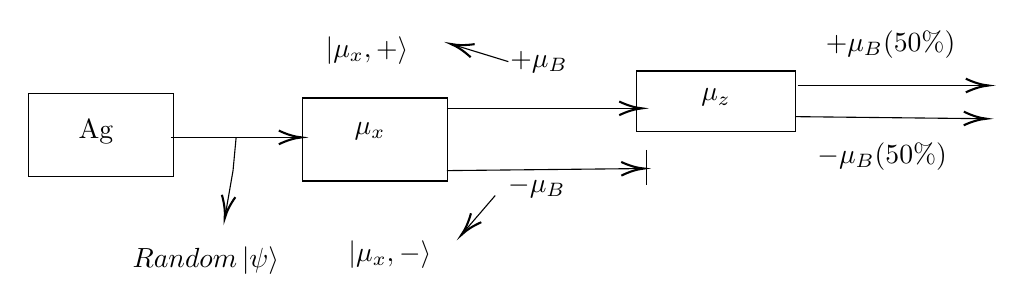
\begin{tikzpicture}[x=0.75pt,y=0.75pt,yscale=-1,xscale=1]
	%uncomment if require: \path (0,300); %set diagram left start at 0, and has height of 300

	%Shape: Rectangle [id:dp04190827497470195]
	\draw   (17,116) -- (87,116) -- (87,156) -- (17,156) -- cycle ;
	%Shape: Rectangle [id:dp571128877254538]
	\draw   (149,118) -- (219,118) -- (219,158) -- (149,158) -- cycle ;
	%Straight Lines [id:da9805949304809836]
	\draw    (85.67,137) -- (146.67,137) ;
	\draw [shift={(148.67,137)}, rotate = 180] [color={rgb, 255:red, 0; green, 0; blue, 0 }  ][line width=0.75]    (10.93,-3.29) .. controls (6.95,-1.4) and (3.31,-0.3) .. (0,0) .. controls (3.31,0.3) and (6.95,1.4) .. (10.93,3.29)   ;
	%Straight Lines [id:da5875299359536541]
	\draw    (218.67,123) -- (310.67,123) ;
	\draw [shift={(312.67,123)}, rotate = 180] [color={rgb, 255:red, 0; green, 0; blue, 0 }  ][line width=0.75]    (10.93,-3.29) .. controls (6.95,-1.4) and (3.31,-0.3) .. (0,0) .. controls (3.31,0.3) and (6.95,1.4) .. (10.93,3.29)   ;
	%Straight Lines [id:da09397377676465912]
	\draw    (218.67,153) -- (259.69,152.57) -- (311.67,152.02) ;
	\draw [shift={(313.67,152)}, rotate = 179.4] [color={rgb, 255:red, 0; green, 0; blue, 0 }  ][line width=0.75]    (10.93,-3.29) .. controls (6.95,-1.4) and (3.31,-0.3) .. (0,0) .. controls (3.31,0.3) and (6.95,1.4) .. (10.93,3.29)   ;
	%Shape: Rectangle [id:dp3443899665830352]
	\draw   (310,105) -- (386.67,105) -- (386.67,134) -- (310,134) -- cycle ;
	%Straight Lines [id:da0016748392119485533]
	\draw    (314.67,143) -- (314.67,160) ;
	%Straight Lines [id:da5799938405144656]
	\draw    (387.67,112) -- (477.67,112) ;
	\draw [shift={(479.67,112)}, rotate = 180] [color={rgb, 255:red, 0; green, 0; blue, 0 }  ][line width=0.75]    (10.93,-3.29) .. controls (6.95,-1.4) and (3.31,-0.3) .. (0,0) .. controls (3.31,0.3) and (6.95,1.4) .. (10.93,3.29)   ;
	%Straight Lines [id:da256275390497529]
	\draw    (387,127) -- (476.67,127.98) ;
	\draw [shift={(478.67,128)}, rotate = 180.63] [color={rgb, 255:red, 0; green, 0; blue, 0 }  ][line width=0.75]    (10.93,-3.29) .. controls (6.95,-1.4) and (3.31,-0.3) .. (0,0) .. controls (3.31,0.3) and (6.95,1.4) .. (10.93,3.29)   ;
	%Straight Lines [id:da7235598208942111]
	\draw    (117.17,137) -- (115.67,153) -- (112.01,174.03) ;
	\draw [shift={(111.67,176)}, rotate = 279.87] [color={rgb, 255:red, 0; green, 0; blue, 0 }  ][line width=0.75]    (10.93,-3.29) .. controls (6.95,-1.4) and (3.31,-0.3) .. (0,0) .. controls (3.31,0.3) and (6.95,1.4) .. (10.93,3.29)   ;
	%Straight Lines [id:da567888731118668]
	\draw    (248.33,100.5) -- (234.93,96.38) -- (222.58,92.59) ;
	\draw [shift={(220.67,92)}, rotate = 17.08] [color={rgb, 255:red, 0; green, 0; blue, 0 }  ][line width=0.75]    (10.93,-3.29) .. controls (6.95,-1.4) and (3.31,-0.3) .. (0,0) .. controls (3.31,0.3) and (6.95,1.4) .. (10.93,3.29)   ;
	%Straight Lines [id:da6159475989059393]
	\draw    (242,165) -- (226.97,182.48) ;
	\draw [shift={(225.67,184)}, rotate = 310.68] [color={rgb, 255:red, 0; green, 0; blue, 0 }  ][line width=0.75]    (10.93,-3.29) .. controls (6.95,-1.4) and (3.31,-0.3) .. (0,0) .. controls (3.31,0.3) and (6.95,1.4) .. (10.93,3.29)   ;

	% Text Node
	\draw (40,127) node [anchor=north west][inner sep=0.75pt]   [align=left] {Ag};
	% Text Node
	\draw (173,128.4) node [anchor=north west][inner sep=0.75pt]    {$\mu _{x}$};
	% Text Node
	\draw (340,112.4) node [anchor=north west][inner sep=0.75pt]    {$\mu _{z}$};
	% Text Node
	\draw (248,94.4) node [anchor=north west][inner sep=0.75pt]    {$+\mu _{B}$};
	% Text Node
	\draw (247,154.4) node [anchor=north west][inner sep=0.75pt]    {$-\mu _{B}$};
	% Text Node
	\draw (400,84.4) node [anchor=north west][inner sep=0.75pt]    {$+\mu _{B}( 50\%)$};
	% Text Node
	\draw (396,138.4) node [anchor=north west][inner sep=0.75pt]    {$-\mu _{B}( 50\%)$};
	% Text Node
	\draw (66,188.4) node [anchor=north west][inner sep=0.75pt]    {$Random\ket{\psi }$};
	% Text Node
	\draw (159,87.4) node [anchor=north west][inner sep=0.75pt]    {$\ket{\mu _{x} ,+}$};
	% Text Node
	\draw (170,185.4) node [anchor=north west][inner sep=0.75pt]    {$\ket{\mu _{x} ,-}$};


\end{tikzpicture}

在这幅图当中,我们可以这样定义态矢量
\begin{align*}
	\ket{\mu_z,+}=\ket{+}=\ket{0} \\
	\ket{\mu_z,-}=\ket{-}=\ket{1} \\
	\mu_B=\frac{e\hbar}{2mc}
\end{align*}

根据这个级联的Stern-Gerlach实验,我们可以得到
\begin{align*}
	\ket{\mu_x,+}              & =C_+\ket{0}+C_-\ket{1}                                                                                                              \\
	|C_+|^2                    & =|C_-|^2=0\frac{1}{2}                                                                                                               \\
	\Rightarrow  \ket{\mu_x,+} & =\frac{1}{\sqrt{2}}\left(e^{i\alpha_1}\ket{0}+e^{i\beta_1}\ket{1}\right)=\frac{1}{\sqrt{2}}\left(\ket{0}+e^{i\beta_1}\ket{1}\right)
\end{align*}

同理,我们可以得到$\ket{\mu_x,-}$
\begin{align*}
	\ket{\mu_x,-}=\frac{1}{\sqrt{2}}\left(\ket{0}+e^{i\gamma_1}\ket{1}\right)
\end{align*}

利用条件
\begin{align*}
	\braket{\mu_x,+}{\mu_x,-}=0
\end{align*}

可以得到
\begin{align*}
	 & e^{i\beta_1}=-e^{i\gamma_1}                                                               \\
	 & \Rightarrow \ket{\mu_x,\pm}=\frac{1}{\sqrt{2}}\left(\ket{0}\pm e^{i\beta_1}\ket{1}\right)
\end{align*}

同理,可以得到
\begin{align*}
	\ket{\mu_y,\pm}=\frac{1}{\sqrt{2}}\left(\ket{0}\pm e^{i\beta_2}\ket{1}\right)
\end{align*}

我们根据正交性
\begin{align*}
	 & \braket{\mu_x,\pm}{\mu_y,\pm}=0            \\
	 & \Rightarrow e^{i\beta_2}=\pm ie^{i\beta_1}
\end{align*}

于是,可以化简得到
\begin{align*}
	\ket{\mu_x,+} & =\frac{1}{\sqrt{2}}\left(\ket{0}+\ket{1}\right)=\frac{1}{\sqrt{2}}
	\begin{pmatrix}
		1 \\
		1
	\end{pmatrix}                                                                             \\
	\ket{\mu_x,-} & =\frac{1}{\sqrt{2}}\left(\ket{0}-\ket{1}\right)=\frac{1}{\sqrt{2}}
	\begin{pmatrix}
		1 \\
		-1
	\end{pmatrix}                                                                             \\
	\ket{\mu_y,+} & =\frac{1}{\sqrt{2}}\left(\ket{0}\pm i\ket{1}\right)=\pm\frac{1}{\sqrt{2}}
	\begin{pmatrix}
		1 \\
		i
	\end{pmatrix}                                                                             \\
	\ket{\mu_y,-} & =\frac{1}{\sqrt{2}}\left(\ket{0}\mp  i\ket{1}\right)=\pm\frac{1}{\sqrt{2}}
	\begin{pmatrix}
		1 \\
		-i
	\end{pmatrix}                                                                             \\
\end{align*}

最后我们可以得到
\begin{align*}
	\hat{\mu}_z=\mu_0\left(\ket{0}\bra{0}-\right)
\end{align*}





\section{量子多体系统}
这也就是说,将原来的波函数进行改写
\begin{align*}
	\psi(x,t)\longrightarrow \psi(x_1,x_2,t)
\end{align*}

这一点,表征在空间中就是指我们将两个粒子各自所在的两个希尔伯特空间$\mathcal{H}_1,\mathcal{H}_2$做了一个张量积$\mathcal{H}=\mathcal{H}_1\otimes \mathcal{H}_2$


\subsection{张量积的性质}
\begin{enumerate}
	\item 标量性:\[(\alpha\ket{\psi_1})\otimes\bra{\psi_2}=\alpha(\ket{\psi_1}\otimes\bra{\psi_2})\]
	\item 线性性:
	      \begin{align*}
		      (\ket{\psi_1}_1+\ket{\psi_2}_1)\otimes \ket{\psi_3}                & =\ket{\psi_1}\otimes\ket{\psi_3}+\ket{\psi_2}\otimes\ket{\psi_3}                            \\
		      \ket{\psi_3}\otimes(\ket{\psi_1}+\ket{\psi_2})                     & =\ket{\psi_3}\otimes\ket{\psi_1}+\ket{\psi_3}\otimes\ket{\psi_2}                            \\
		      (\alpha\ket{\psi_1}+\beta\ket{\psi_2})\otimes (\gamma\ket{\psi_3}) & =(\alpha\gamma)\ket{\psi_1}\otimes\ket{\psi_3}+(\beta\gamma)\ket{\psi_2}\otimes\ket{\psi_3}
	      \end{align*}
	\item 对于一个纠缠态(entangled state)所描述的量子态是一群不能够被互相单独描述的粒子所对应的态(包括粒子被分开有很长一段距离)
	      \begin{align*}
		                  & \ket{\psi}_{1\otimes 2}\in V_1\otimes V_2               \\
		      \Rightarrow & \ket{\psi}_{1\otimes 2}=\ket{\psi}_1\otimes\ket{\psi}_2
	      \end{align*}

	      如果对于量子态$\ket{\psi}_{1\otimes 2}$并不能够被写成这样的形式,那么我们称之为纠缠态(entangled state)

	      假设对于一个算符存在两个纠缠态$\ket{v_1}_1,\ket{v_2}_1\in V_1$,
	      以及$\ket{w_1}_2,\ket{w_2}_2\in V_2$
	      \begin{enumerate}
		      \item 如果粒子1的态矢量可以写为
		            \begin{align*}
			            \ket{\psi}_1=a\ket{v_1}_1+b\ket{v_2}_1
		            \end{align*}
		            如果粒子2的态矢量可以写为
		            \begin{align*}
			            \ket{\phi}_2=c\ket{w_1}_2+d\ket{w_2}_2
		            \end{align*}
		            那么这两个粒子所组成的态矢量$(\ket{\psi}_1\otimes\ket{\phi}_2)$,是非纠缠态的
		      \item 双粒子态为纠缠态的粒子
		            \begin{itemize}
			            \item
			                  \begin{align*}
				                  \ket{\psi}_{1\otimes 2}=a\ket{v_1}_1\otimes c\ket{w_1}_2+b\ket{v_2}_1\otimes d\ket{w_2}_2
			                  \end{align*}
			            \item
			                  \begin{align*}
				                  \ket{\psi}_{1\otimes 2}=a\ket{v_1}_1\otimes d\ket{w_2}_2 +b\ket{v_2}_1\otimes c\ket{w_1}_2
			                  \end{align*}
		            \end{itemize}
	      \end{enumerate}
	\item 零矢量$\ket{0}$
	      \begin{align*}
		      \ket{0}_1\otimes\ket{\phi}_2=\ket{\psi}_1\otimes\ket{0}_2
	      \end{align*}
	\item 如果$\displaystyle\ket{\psi}_1=\sum_{i}c_i\ket{v_i}_1,\ket{\phi}_2=\sum_{j}d_j\ket{w_j}_2$,那么
	      \begin{align*}
		      \ket{\psi}_1\otimes\ket{\phi}_2 & =\sum_{i,j}c_id_j\ket{v_i}_1\otimes\ket{w_j}_2  \\
		                                      & = \sum_{i,j}f_{ij}\ket{v_i}_1\otimes\ket{w_j}_2
	      \end{align*}
	\item 两个空间做张量积之后的维数等于两个空间的维数之积
	      \begin{align*}
		      \dim{}(\mathcal{H}_1\otimes\mathcal{H}_2)=\dim{\mathcal{H}_1}\cdot\dim{\mathcal{H}_2}
	      \end{align*}
	\item 假设算符$A$在$V_1$中,算符$B$在$V_2$中,并且他们有
	      \begin{align*}
		      A\ket{v_i}_1 & =a_i\ket{v_i}_1 \\
		      B\ket{w_j}_2 & =b_j\ket{w_j}_2
	      \end{align*}
	      那么算符的张量积$A\otimes B$为
	      \begin{align*}
		      A\otimes B \ket{v_i}_1\otimes \ket{w_j}_2 & =a_ib_j\ket{v_i}_1\otimes \ket{w_j}_2
	      \end{align*}
	      因此,我么可以将两个空间中的算符之间的张量积写为
	      \begin{align*}
		      A\otimes B & =(A\otimes I)(I\otimes B) \\
		                 & =(I\otimes A)(B\otimes I)
	      \end{align*}
	      这将可以导出张量积的对易性(对于两个空间中的算符的作用是互不干扰的)
	      \begin{align*}
		      [A\otimes I,I\otimes B]=0
	      \end{align*}
	      由此,我们还可以进一步直观的得到
	      \begin{align*}
		      (A\otimes B)(C\otimes D)=AC\otimes BD
	      \end{align*}
	\item
	      \begin{align*}
		      \ket{\psi}_1=
		      \begin{pmatrix}
			      \psi_1 \\ \psi_2
		      \end{pmatrix}\in V_1
		      ,\ket{\phi}_2=
		      \begin{pmatrix}
			      \phi_1 \\ \phi_2\\ \phi_3
		      \end{pmatrix}\in V_2
	      \end{align*}
	      于是我们可以得到这两个的张量积为
	      \begin{align*}
		      \ket{\psi}_1\otimes\ket{\phi}_2
		      =
		      \begin{pmatrix}
			      \psi_1\otimes\ket{\phi}_2 \\ \psi_2\otimes\ket{\phi}_2
		      \end{pmatrix}
		      =
		      \begin{pmatrix}
			      \psi_1\phi_1 \\\psi_1\phi_2\\\psi_1\phi_3\\\psi_2\phi_1\\\psi_2\phi_2\\\psi_2\phi_3
		      \end{pmatrix}
	      \end{align*}
	      另外还有一个例子,
	      \begin{align*}
		      A=\pmtwo{A_{11}}{A_{12}}{A_{21}}{A_{22}}\in V_1,
		      B=\pmthree{B_{11}}{B_{12}}{B_{13}}{B_{21}}{B_{22}}{B_{23}}{B_{31}}{B_{32}}{B_{33}}\in V_2
	      \end{align*}
	      他们的张量积为
	      \begin{align*}
		      A\otimes B=
		      \begin{pmatrix}
			      A_{11}B & A_{12}B \\
			      A_{21}B & A_{22}B
		      \end{pmatrix}
	      \end{align*}
	\item 给定三个波函数$\displaystyle\ket{\phi}_{1\otimes 2},\ket{\psi}_{1\otimes 2},\ket{\eta}_{1\otimes 2}\in V_1\otimes V_2$那么将会有如下的性质:
	      \begin{enumerate}
		      \item \[\braket{\psi+\phi}{\eta}_{1\otimes2}=\braket{\psi}{\eta}+\braket{\phi}{\eta}_{1\otimes2}\]
	      \end{enumerate}
	      剩下的性质与之前在一个空间中的一摸一样,就不再一一列举了

	      如果这时候我给定两组基,分别是它们对应的空间中的正交归一基,$\ket{v_i}_1\in V_1$,$\ket{w_j}_2 \in V_2$

	      那么将会有
	      \begin{align*}
		      (\bra{v_i}_1\otimes\ket{w_j}_2)(\ket{v_k}_1\otimes\ket{w_l}_2) & =\braket{v_i}{v_k}\braket{w_j}{w_l} \\
		                                                                     & =\delta_{ik}\delta_{jl}
	      \end{align*}

	      将其应用至无穷维空间的情况,可以得到
	      \begin{align*}
		      (\bra{\psi}_1\otimes \bra{\phi}_2)(\ket{\eta}_1\otimes \ket{\xi}_2)
	      \end{align*}

	      所以,如果两个基是正交的,那么这两个基的共轭转置也是正交的。
\end{enumerate}


\subsection{量子多体系统的薛定谔方程}
\begin{align*}
	i\hbar\frac{\partial}{\partial t}\psi(x_1,x_2,t)                                                                                                      & = H\psi(x_1,x_2,t)                                 \\
	\left[-\frac{\hbar^2}{2m_1}\frac{\partial^2}{\partial x_1^2}-\frac{\hbar^2}{2m_2}\frac{\partial^2}{\partial x_2^2}+V(x_1,x_2,t)\right]\psi(x_1,x_2,t) & = i\hbar\frac{\partial}{\partial t}\psi(x_1,x_2,t)
\end{align*}

接下来让我们分析一下这个方程,这将会是求解的关键
\begin{enumerate}
	\item[case1:] $V(x_1,x_2)=V(x_1)+V(x_2)$ 这其实也意味着这两个粒子是完全没有相互作用的
	\item[case2:] $V(x_1,x_2)=V(x_1-x_2)$这个问题可以转化为一个中心力场问题

	      对于这种问题,直接假设$\displaystyle x=x_1-x_2,x_{cm}=\frac{m_1x_1+m_2x_2}{m_1+m_2}$,没错就是质心系,那么我们就可以直接去使用约化质量$\mu=m_1m_2/(m_1+m_2)$来进行运算了

	      可以得到,哈密顿量为
	      \begin{align*}
		      H(x_1p_1;x_2,p_2) & =H(x_{cm},p_{cm};x,p)                              \\
		                        & =H_{cm}+H_{relative}                               \\
		                        & =\frac{p_{cm}^2}{2(m_1+m_2)}+\frac{p^2}{2\mu}+V(x)
	      \end{align*}

	      波函数改写为
	      \begin{align*}
		      \psi(x_1,x_2)=\psi_{cm}(x_{cm})\psi(x) \\
		      =\frac{1}{\sqrt{2\pi\hbar}}e^{\frac{i}{\hbar}p_{cm}x_{cm}}\psi(x)
	      \end{align*}
	      将其写为本征方程形式
	      \begin{align*}
		      H\ket{\psi}                     & =E\ket{\psi}                                            \\
		      (H_{cm}+H_{relative})\ket{\psi} & =(E+E_r)\ket{\psi}                                      \\
		      (H_{cm}+H_{relative})\ket{\psi} & =\left(\frac{p_{cm^2}}{2(m_1+m_2)}+E_r\right)\ket{\psi}
	      \end{align*}
\end{enumerate}


\subsection{全同粒子}
全同粒子这个名词所赋予的是微观粒子的不可区分性,这体现在粒子的内禀属性:质量(mass)、电荷(charge)、自旋(spin)、颜色(color)等等,而在这些属性当中,自旋是非常重要的一个属性,我们也是依靠自旋将粒子分为了两类:玻色子和费米子。

\begin{enumerate}
	\item 玻色子(Boson):自旋为整数的粒子,比如光子、声子等等
	\item 费米子(Fermion):自旋为半整数的粒子,比如电子、质子、中子等等
\end{enumerate}

接下来我们考虑一个$n$粒子体系,那么它的态矢量所在的空间写成
\begin{align*}
	\mathbb{H}^{\otimes N} =\mathbb{H}_1\otimes\mathbb{H}_2\otimes\cdots\otimes\mathbb{H}_n
\end{align*}

而这个$n$粒子体系的态矢量,根据我们之前所学到的几大公设,这个应该是可以被展开为每一个空间中的基矢量的张量积的任意线性组合,如下
\begin{align*}
	\ket{\psi}=\sum_{j}^n C_j \left(\ket{u_1}\otimes\ket{\u_2}\otimes\cdots\otimes\ket{u_n}\right)
\end{align*}

但是事实上,并不可以这样做,我们会出现一个交换简并(Exchange Degeneray)的问题(即我们可以将任意的两个空间的基矢量的张量积进行交换,但是这样做很显然是不该出现的)

\begin{example}
	接下来举个例子:对于一个(two-spin)体系$\ket{+},\ket{-}$,如两个电子的体系,我们可以写成这样的形式

	Basis:
	\begin{align*}
		\ket{+}\otimes\ket{-},\ket{-}\otimes\ket{+}
	\end{align*}

	那么对于这个体系的态矢量将被写成
	\begin{align*}
		\ket{\psi}=\alpha\ket{+}\otimes\ket{-}+\beta\ket{-}\otimes\ket{+}
	\end{align*}

	但是这样做对吗?我们来验证一下

	此时如果我们想要尝试测量一下他们x方向上的自旋的概率

	首先是给出我们的测量算符
	\begin{align*}
		\ket{x,+} & =\frac{1}{\sqrt{2}}\left(\ket{+}+\ket{-}\right) \\
		\ket{x,-} & =\frac{1}{\sqrt{2}}\left(\ket{+}-\ket{-}\right)
	\end{align*}

	于是,我们可以得到在这个双自旋体系在x方向上的测量算符
	\begin{align*}
		\ket{x,+}\otimes\ket{x,-} & =\frac{1}{2}\left(\ket{+}\otimes\ket{+}-\ket{+}\otimes\ket{-}+\ket{-}\otimes\ket{+}-\ket{-}\otimes\ket{-}\right) \\
		\ket{x,-}\otimes\ket{x,+} & =\frac{1}{2}\left(\ket{+}\otimes\ket{+}+\ket{+}\otimes\ket{-}-\ket{-}\otimes\ket{+}-\ket{-}\otimes\ket{-}\right)
	\end{align*}

	接下来,将这个测量算符带入到我们的概率计算公式中
	\begin{align*}
		P_x(+,-) & =\left|\bra{+,x}\braket{-,x}{\psi}\right|^2 \\
		         & =\left|\right|^2
	\end{align*}
\end{example}





如果仍然考虑两个粒子$\ket{ab}$,那么有这样的关系
\begin{align*}
	\ket{ab}=\ket{x_1=x_a,m_1=m_a;x_2=x_b,m_2=m_b}
\end{align*}

同理
\begin{align*}
	\ket{ba}=\ket{x_1=x_b,m_1=m_b;x_2=x_a,m_2=m_a}
\end{align*}

那么考虑一个态
\begin{align*}
	\ket{\psi(a,b)}=\beta\ket{ab}+\gamma\ket{ba}
\end{align*}

在考虑一个置换算符$P$,使得有关系
\begin{align*}
	P\ket{\psi(a,b)} & =\beta\ket{ba}+\gamma\ket{ab}         \\
	                 & =\alpha(\beta\ket{ab}+\gamma\ket{ba})
\end{align*}
这也就是说
\begin{align*}
	\begin{cases}
		\beta  & =\alpha\gamma \\
		\gamma & =\alpha\beta
	\end{cases}
\end{align*}

通过求解,我们可以得到$\alpha=\pm 1$,而$\beta =\pm \gamma$
通过这个,我们将定义出两种粒子

\begin{enumerate}
	\item[(1)] boson对称\[P\ket{\psi_s}=\ket{ab}+\ket{ba}\]
	\item[(2)] fermi反对称\[P\ket{\psi_f}=\ket{ab}-\ket{ba}\]
\end{enumerate}

\paragraph{泡利不相容原理}
两个可分辨的玻色子可以处于同一量子态,两个可分辨的费米子不能处在同一量子态

那么我们直接来验证一下
\begin{align*}
	\ket{\psi_s^a} & =\ket{aa}+\ket{aa}   \\
	\ket{\psi_f^a} & =\ket{aa}-\ket{aa}=0
\end{align*}

很明显,费米子在这个时候直接变成$0$了

当然,对于玻色子,我们也可以写成函数的形式
\begin{align*}
	\psi_{s}(x_1,x_2)=\frac{1}{\sqrt{2}}\left[\psi_1(x_1)\psi_2(x_2)+\psi_2(x_1)\psi_2(x_1)\right]
\end{align*}

写成态势也可以是这样的
\begin{align*}
	\ket{\psi_s(x_1,x_2)} & =\frac{1}{\sqrt{2}}\left[\ket{\psi_1(x_1)}_1\otimes\ket{\psi_2(x_2)}_2+\ket{\psi_2(x_1)}_1\otimes\ket{\psi_1(x_2)}_2\right] \\
	                      & =\frac{1}{\sqrt{2}}\left[\ket{\psi_1(x_1)}\ket{\psi_2(x_2)}+\ket{\psi_2(x_1)}\ket{\psi_1(x_2)}\right]
\end{align*}

对于费米子这种反对称的,我们也同样的可以写成
\begin{align*}
	\psi_{a}(x_1,x_2) & =\frac{1}{\sqrt{2}}\left[\psi_1(x_1)\psi_2(x_2)-\psi_2(x_1)\psi_2(x_1)\right]                                       \\
	                  & =\frac{1}{\sqrt{2}}\left[\ket{\psi_1(x_1)}\otimes\ket{\psi_2(x_2)}-\ket{\psi_2(x_1)}\otimes\ket{\psi_1(x_2)}\right] \\
	                  & =\frac{1}{\sqrt{2}}\vmtwo{\psi_1(x_1)}{\psi_1(x_2)}{\psi_2(x_1)}{\psi_2(x_2)}
\end{align*}

下面我们来验证一下归一化条件,
\begin{align*}
	\braket{\psi_{s/a}(x_1,x_2)}{\psi_{s/a}(x_1,x_2)} & =\left\{\frac{1}{\sqrt{2}}\left[\bra{\psi_1(x_1)}\bra{\psi_2(x_2)\pm\bra{\psi_2(x_1)\bra{\psi_1(x_2)}}}\right]\right\}      \\
	                                                  & \times\left\{\frac{1}{\sqrt{2}}\left[\ket{\psi_1(x_1)}\ket{\psi_2(x_2)}\pm\ket{\psi_2(x_1)}\ket{\psi_1(x_2)}\right]\right\} \\
	                                                  & =
\end{align*}

很显然,上面只讨论了两个粒子的系统,下面让我们尝试一下三个粒子的系统,其波函数仍然可以写为
\begin{align*}
	\ket{\psi_s(x_1,x_2,x_3)} & =                                                                                                                                                 \\
	\ket{\psi_a(x_1,x_2,x_3)} & =\frac{1}{\sqrt{3!}}\vmthree{\psi_1(x_1)}{\psi_1(x_2)}{\psi_1(x_3)}{\psi_2(x_1)}{\psi_2(x_2)}{\psi_2(x_3)}{\psi_3(x_1)}{\psi_3(x_2)}{\psi_3(x_3)}
\end{align*}

\subsection{量子多体系统的一维无限位能阱}
对于一个粒子的系统,我们在之前就已经有涉及到
首先,如果是一个两粒子的系统(没有相互作用),
\begin{enumerate}
	\item[可分辨粒子]
	      \begin{align*}
		      \psi_{n_1,n_2}(x_1,x_2) & =\psi_{n_1}(x_1)\psi_{n_2}(x_2)                                \\
		                              & =\frac{2}{L}\sin{\frac{n_1\pi}{L}x_1}\sin{\frac{n_2\pi}{L}x_2} \\
		      E_{n_1,n_2}             & =(n_1^2+n_2^2)E_1
	      \end{align*}

	      很显然,这个地方,一个能谱可以对应到两个不同的量子态,因此是简并的
	\item[玻色子]
	      \begin{align*}
		      \psi_{n_1,n_2}^s & =\frac{1}{\sqrt{2!}}\left[\psi_{n_1}(x_1)\psi_{n_2}(x_2)+\psi_{n_2}(x_1)\psi_{n_1}(x_2)\right] \\
		      E_{n_1,n_2}      & =(n_1^2+n_2^2)E_1
	      \end{align*}
	\item[费米子]
	      \begin{align*}
		      \psi^a(x_1,x_2) & =\frac{1}{\sqrt{2}}\left[\psi_1(x_1)\psi_2(x_2)-\psi_2(x_1)\psi_2(x_1)\right] \\
		      E_{n_1,n_2}     & =(n_1^2+n_2^2)E_1
	      \end{align*}
	      但这在费米子中将会更加特殊,因为费米子的$n_1,n_2$是不可以相同的,这也就意味着,当$n_1=1$时,$n_2=2$,也就是说,两个费米子系统的基态的能量将会是$E_g=5E_1$
\end{enumerate}

\subsection{期望值}
首先计算一下两个可区分粒子的期望值
\begin{align*}
	\expectation{(x_1-x_2)^2} & =\expectation{x_1^2-2x_1x_2+x_2^2}                                                                                   \\
	                          & =\expectation{x_1^2}-\expectation{2x_1x_2}+\expectation{x_2^2}                                                       \\
	                          & =\bra{\psi_1(x_1)}x_1^2\ket{\psi_1(x_1)}-2\bra{\psi_1(x_1)}x_1\ket{\psi_1(x_1)}\bra{\psi_2(x_2)}x_2\ket{\psi_2(x_2)} \\
	                          & +\bra{\psi_2(x_2)}x_2^2\ket{\psi_2(x_2)}                                                                             \\
	                          & =\expectation{x_1^2}_{\psi_1}-2\expectation{x_1}_{\psi_1}\expectation{x_2}_{\psi_2}+\expectation{x_2^2}_{\psi_2}
\end{align*}

接下来讨论对于全同粒子的情况,首先还是先写出全同粒子的态
\begin{align*}
	\ket{\psi_{S/A}}(x_1,x_2)=\frac{1}{\sqrt{2!}}\left[\ket{\psi_1(x_1)\psi_2(x_2)\pm\psi_2{x_1}\psi_1(x_2)}\right]
\end{align*}

紧接着开始去计算期望值
\begin{align*}
	\expectation{(x_1-x_2)^2} & =\expectation{x_1^2}_{\psi_1}-2\expectation{x_1}_{\psi_1}\expectation{x_2}_{\psi_2}+\expectation{x_2^2}_{\psi_2}                                                                                   \\
	                          & =\text{回去再补充}                                                                                                                                                                                      \\
	                          & =\frac{1}{2}\left(\expectation{x^2}_{\psi_1}+\expectation{x^2}_{\psi_2}\right)+\frac{1}{2}\left(\expectation{x^2}_{\psi_1}+\expectation{x^2}_{\psi_2}\right)                                       \\
	                          & +\frac{1}{2}\left(\expectation{x^2}_{\psi_1}\expectation{x^2}_{\psi_2}+\expectation{x^2}_{\psi_2}\expectation{x^2}_{\psi_1}\pm2\expectation{x}_{\psi_1\psi_2}\expectation{x}_{\psi_2\psi_1}\right) \\
	                          & =\expectation{x^2}_{\psi_1}+\expectation{x^2}_{\psi_2}-2\expectation{x^2}_{\psi_1}\expectation{x^2}_{\psi_2}\mp \textcolor{red}{2\left|\expectation{x}_{\psi_1\psi_2}\right|^2}
\end{align*}

从结果上来看,我们可以得到如下的总结:\textbf{相对于两个可分辨的粒子之间的距离的期望值,两个玻色子之间的距离的期望值要比可区分粒子的期望值要小一点点,而两个费米子之间的距离的期望值要比可分辨粒子的期望值要大一点点}
\newpage
\section{不含时微扰理论}
所谓的微扰,就是在解决一个问题的时候,我们发现这个问题与我们之前所解决的问题并没有很大的差别,只是可能多了一点点小的突起,那么我们就将这个小的突起当作为这个系统的微扰。

\subsection{非简并微扰理论}

\subsubsection{微扰理论一般公式推导}

假设对于某个情况(如图),我们将会有本征方程
\begin{align*}
	H\ket{\psi_n}=E\ket{\psi_n}
\end{align*}

\begin{figure}[hbtp]
	\centering
	\includegraphics[width=0.5\textwidth]{figure/存在微扰的一维无限位能阱.png}
	\caption{微扰}
\end{figure}



但是我们此时又有一个系统,是我们非常熟悉的(如图),对于这种情况的本征方程,我们列为
\begin{align*}
	H^0\ket{\psi_n^0}=E^0\ket{\psi_n^0}
\end{align*}

\begin{figure}
	\centering
	\includegraphics[width=0.5\textwidth]{figure/一维无限位能阱.png}
	\caption{无微扰}
\end{figure}
此时,我们将哈密顿量写为
\begin{align*}
	H=H^0+ H^1
\end{align*}

于是我们可以把含有围绕的一维无限位能阱问题的本征方程写为
\begin{align*}
	H\ket{\psi_n}=(H^0+H^1)\ket{\psi_n}=E_n\ket{\psi_n}
\end{align*}

于是,我们也可以将能谱以及波函数做微扰展开为
\begin{align*}
	E_n          & =E_n^0+\lambda E_n^1+\lambda^2 E_n^2+\cdots\quad\quad \lambda\in[0,1]                          \\
	\ket{\psi_n} & =\ket{\psi_n^0}+\lambda\ket{\psi_n^1}+\lambda^2\ket{\psi_n^2}+\cdots\quad\quad \lambda\in[0,1]
\end{align*}

OK!现在将其代入到我们之前得出的本征方程中
\begin{align*}
	(H^0+H^1)\ket{\psi_n}                                             & =E_n\ket{\psi_n}                                                                                 \\
	(H^0+H^1)\left(\ket{\psi_n^0}+\lambda\ket{\psi_n^1}+\cdots\right) & =\left(E_n^0+\lambda E_n^1+\cdots\right)\left(\ket{\psi_n^0}+\lambda\ket{\psi_n^1}+\cdots\right)
\end{align*}

接下来我们对这个式子进行整合,可以得到
\begin{align*}
	  & H\psi_n^0+\lambda\left(H^0\psi_n^1+H^1\psi_n^0\right)+\lambda^2\left(H^0\psi_n^2+H^1\psi_n^1\right)+\cdots                           \\
	= & E_n^0\psi_n^0+\lambda\left(E_n^0\psi_n^1+E_n^1\psi_n^0\right)+\lambda^2\left(E_n^0\psi_n^2+E_n^1\psi_n^1+E_n^2\psi_n^0\right)+\cdots
\end{align*}

在这个方程当中,对于零级项($\lambda^0$)
\begin{align*}
	H\psi_n^0=E_n^0\psi_n^0
\end{align*}

对于一级项($\lambda$)
\begin{align*}
	H^0\psi_n^1+H^1\psi_n^0=E_n^0\psi_n^1+E_n^1\psi_n^0
\end{align*}

对于二级项($\lambda^2$)
\begin{align*}
	H^0\psi_n^2+H^1\psi_n^1=E_n^0\psi_n^2+E_n^1\psi_n^1+E_n^2\psi_n^0
\end{align*}

\subsubsection{一级近似理论}
顾名思义,就是对我们在上一节当中通过微扰展开得到的一级项进行一个计算,毕竟零级项我们在之前便已经计算过,下面我们给出一级项所带来的方程
\begin{align*}
	H^0\psi_n^1+H^1\psi_n^0=E_n^0\psi_n^1+E_n^1\psi_n^0
\end{align*}

\paragraph{能量的一级修正}直接对其求内积,可以得到
\begin{align*}
	\bra{\psi_n^0}H^0\ket{\psi_n^1}+\bra{\psi_n^0}H^1\ket{\psi_n^0} & =\bra{\psi_n^0}E_n^0\ket{\psi_n^1}+\bra{\psi_n^0}E_n^1\ket{\psi_n^0} \\
	\bra{\psi_n^0}H^1\ket{\psi_n^0}                                 & =E_n^1\braket{\psi_n^0}{\psi_n^0}                                    \\
	\bra{\psi_n^0}H^1\ket{\psi_n^0}                                 & =E_n^1
\end{align*}

于是,我们得到了一级修正所得到的一个基本结果
\begin{equation*}
	\bra{\psi_n^0}H^1\ket{\psi_n^0}=E_n^1
\end{equation*}

这个等式可以说是一个量子力学当中非常重要的方程,他也说明了一点:\textbf{能量的一级修正就是微扰项在无微扰态中的期望值}

\paragraph{波函数的一级修正}将我们在上一节当中得到的一级项方程进行一个移项,得到
\begin{align*}
	\left(H^0-E_n^0\right)\psi_n^1=-\left(H^1-E_n^1\right)\psi_n^0
\end{align*}

此时的方程是一个关于$\psi_n^1$的非齐次偏微分方程,由于无微扰的波函数是完备的,因此我们可以将$\psi_n^1$表示为他们的线性组合:
\begin{align*}
	\psi_n^1 & =\sum_{m\neq n}c_m^{(n)}\psi_m^0
\end{align*}

接下来带入到方程当中,可以得到
\begin{align*}
	\sum_{m\neq n}\left(H^0-E_n^0\right)c_m^{(n)}\psi_m^0   & =-\left(H^1-E_n^1\right)\psi_n^0 \\
	\sum_{m\neq n}\left(E_m^0-E_n^0\right)c_m^{(n)}\psi_m^0 & =-\left(H^1-E_n^1\right)\psi_n^0
\end{align*}

取一个$\psi_l^0$与上式做内积
\begin{align*}
	\sum_{m\neq n}\left(H^0-E_n^0\right)c_m^{(n)}\braket{\psi_l^0}{\psi_m^0} & =-\left(H^1-E_n^1\right)\braket{\psi_l^0}{\psi_m^0} \\
\end{align*}

如果$l=n$,那么左边为$0$,那么我们将可以得到
\begin{equation*}
	\bra{\psi_n^0}H^1\ket{\psi_n^0}=E_n^1
\end{equation*}

反之,如果$l\neq n$,我们会有
\begin{align*}
	\left(E_l^0-E_n^0\right)c_l^{(n)}=-\bra{\psi_l^0}H^1\ket{\psi_n^0}
\end{align*}

即,
\begin{align*}
	c_m^{(n)}=-\dfrac{\bra{\psi_m^0}H^1\ket{\psi_n^0}}{E_m^0-E_n^0}
\end{align*}

所以有,
\begin{align*}
	\psi_n^1=-\sum_{m\neq n}\dfrac{\bra{\psi_m^0}H^1\ket{\psi_n^0}}{E_m^0-E_n^0}\psi_m^0
\end{align*}

这是非简并的情况。

\paragraph{能量的二级修正}
同样是没有什么奇怪的,都是计算,将$\psi_n^0$与二级近似方程做一个内积,即,
\begin{align*}
	\bra{\psi_n^0}\left(H^0\psi_n^2+H^1\psi_n^1\right)               & =\bra{\psi_n^0}\left(E_n^0\psi_n^2+E_n^1\psi_n^1+E_n^2\psi_n^0\right)                               \\
	E_n^0\braket{\psi_n^0}{\psi_n^2}+\bra{\psi_n^0}H^1\ket{\psi_n^1} & =E_n^0\braket{\psi_n^0}{\psi_n^2}+E_n^1\braket{\psi_n^0}{\psi_n^1}+E_n^2\braket{\psi_n^0}{\psi_n^0}
\end{align*}

同时,我们可以知道
\begin{align*}
	\braket{\psi_n^0}{\psi_n^1}=\sum_{m\neq n}\dfrac{\bra{\psi_m^0}H^1\ket{\psi_n^0}}{E_m^0-E_n^0}\braket{\psi_n^0}{\psi_m^0}=0
\end{align*}

因此,我么可以得出$E_n^2$
\begin{align*}
	\bra{\psi_n^0}H^1\ket{\psi_n^1} & =E_n^2\braket{\psi_n^0}{\psi_n^0}                                                                  \\
	E_n^2                           & =\bra{\psi_n^0}H^1\ket{\psi_n^1}                                                                   \\
	                                & =\sum_{n\neq m}c_m^{(n)}\bra{\psi_n^0}H^1\ket{\psi_m^0}                                            \\
	                                & =\sum_{n\neq m}\dfrac{\bra{\psi_m^0}H^1\ket{\psi_n^0}\bra{\psi_n^0}H^1\ket{\psi_m^0}}{E_n^0-E_m^0} \\
	                                & =\sum_{n\neq m}\dfrac{\left|\bra{\psi_m^0}H^1\ket{\psi_n^0}\right|^2}{E_n^0-E_m^0}
\end{align*}

\subsection{简并微扰理论}
\subsubsection{二重简并}

前面的之后补充

如果我们可以找到一个特定的算符$A$满足以下的条件
\begin{enumerate}
	\item $[H,A]=0$
	\item $[H^1,A]=0$
	\item $\ket{\psi_1^0},\ket{\psi_2^0}$对于算符$A$是非简并的
\end{enumerate}

那么我们可能可以提前找到它的本征值。

\begin{theorem}
	如果算符$A$是哈密顿量$H_1$的厄米算符,并且态$\ket{\phi_1^0},\ket{\phi_2^0}$是算符$A$的本征矢量,且是非简并的
	\begin{align*}
		A\ket{\phi_1^0}=a_1\ket{\phi_1^0} \\
		A\ket{\phi_2^0}=a_2\ket{\phi_2^0}
	\end{align*}

	那么将会有
	\begin{align*}
		\bra{\phi_1^0}H^1\ket{\phi_2^0}=0
	\end{align*}
\end{theorem}

\begin{proof}
	直接假设$[H^1,A]=0$,那么我们将会有
	\begin{align*}
		\Rightarrow \bra{\phi_1^0}[H^1,A]\ket{\phi_2^0} & =0 \\
		\bra{\phi_1^0}H^1A-AH^1\ket{\phi_2^0}           & =0 \\
		(a_1-a_2)\bra{\phi_1^0}H^1\ket{\phi_2^0}        & =0 \\
		\Rightarrow \bra{\phi_1^0}H^1\ket{\phi_2^0}=0
	\end{align*}
\end{proof}

\begin{example}
	考虑一个三维的无限势阱,其势能为
	\begin{align*}
		V(x,y,z)=
		\begin{cases}
			0,     & \quad\quad 0<x<L,0<y<L,0<z<L \\
			\infty & \quad\quad otherwise
		\end{cases}
	\end{align*}
	\begin{solution}
		很显然,一个三维的我们可以将其波函数拆分为$\psi(x,y,z)=\psi_x(x)\psi_y(y)\psi_z(z)$,而我们是知道的对于他们的一维情况,我们有解
		\begin{align*}
			\psi_{x}(x)=\sqrt{\frac{2}{L}}\sin{k_nx},\quad k_n=\frac{2mE}{\hbar^2}
		\end{align*}

		同时,我们也会有能谱
		\begin{align*}
			E_{nx}=\frac{\hbar^2\pi^2}{2mL^2}n_x^2
		\end{align*}

		将其综合起来,我们会有最终的答案
		\begin{align*}
			\psi_{ijk}(x,y,z)=\left(\frac{2}{L}\right)^{\frac{3}{2}}\sin{\frac{n_x\pi}{L}x}\sin{\frac{n_y\pi}{L}y}\sin{\frac{n_z\pi}{L}z} \\
			E_{n ijk}^0=E_{nx}+E_{ny}+E_{nz}=\frac{\hbar^2\pi^2}{2mL^2}\left(n_x^2+n_y^2+n_z^2\right)
		\end{align*}

		可以预见,在能级为1的时候,能量只有一个,但是当能级为2的时候,发生了三重简并

		这个时候,我们加入一个微扰
		\begin{align*}
			H^1=
			\begin{cases}
				V, & \quad\quad 0<x<\frac{L}{2},0<y<\frac{L}{2},0<z<L \\
				0  & \quad\quad otherwise
			\end{cases}
		\end{align*}

		对于基态能量$E_g=E_{111}^0+E_{111}^1$
		\begin{align*}
			E_{111}^1 & =\bra{\psi_{111}^0}H^1\ket{\psi_{111}^0}                                                                                                                                                   \\
			          & =\int_{0}^{\frac{L}{2}} dx\int_{0}^{\frac{L}{2}} dy\int_{0}^{\frac{L}{2}} dz \left[\left(\sin^2{\frac{n_x\pi}{L}x}\sin^2{\frac{n_y\pi}{L}y}\sin^2{\frac{n_z\pi}{L}z}\right)\times V\right] \\
			          & =\frac{V}{4}
		\end{align*}

		因此,我们给出了一阶修正
		\begin{align*}
			E_{111}=\frac{3\hbar^2\pi^2}{2mL}+\frac{V}{4}
		\end{align*}

		接下来我们定义$\psi_{112}^0\equiv\psi_1^0,\psi_{121}^0=\equiv\psi_2^0,\psi_{211}^0\equiv\psi_3^0$
		\begin{align*}
			H^1=
			\begin{pmatrix}
				H_{11}^1 & H_{12}^1 & H_{13}^1 \\
				H_{21}^1 & H_{22}^1 & H_{23}^1 \\
				H_{31}^1 & H_{32}^1 & H_{33}^1
			\end{pmatrix}
		\end{align*}
		通过逐个积分,我们可以有每一个矩阵元的值
		\begin{align*}
			H_{11}^1 & =\int_{0}^{\frac{L}{2}} dx\int_{0}^{\frac{L}{2}} dy\int_{0}^{L} dz \left[\left(\sin^2{\frac{\pi}{L}x}\sin^2{\frac{\pi}{L}y}\sin^2{\frac{2\pi}{L}z}\right)\times V\right] \\
			         & =\frac{V}{4}                                                                                                                                                             \\
			H_{22}^1 & =\int_{0}^{\frac{L}{2}} dx\int_{0}^{\frac{L}{2}} dy\int_{0}^{L} dz \left[\left(\sin^2{\frac{\pi}{L}x}\sin^2{\frac{2\pi}{L}y}\sin^2{\frac{\pi}{L}z}\right)\times V\right] \\
			         & =\frac{V}{4}                                                                                                                                                             \\
			H_{33}^1 & =\int_{0}^{\frac{L}{2}} dx\int_{0}^{\frac{L}{2}} dy\int_{0}^{L} dz \left[\left(\sin^2{\frac{2\pi}{L}x}\sin^2{\frac{\pi}{L}y}\sin^2{\frac{\pi}{L}z}\right)\times V\right] \\
			         & =\frac{V}{4}                                                                                                                                                             \\
			H_{12}^1 & =0                                                                                                                                                                       \\
			H_{13}^1 & =0                                                                                                                                                                       \\
			H_{23}^1 & =\frac{16}{9\pi^2}V
		\end{align*}

		写成将这些值重新放回到矩阵当中,就可以得到
		\begin{align*}
			H^1=\frac{V}{4}
			\begin{pmatrix}
				1 & 0      & 0      \\
				0 & 1      & \kappa \\
				0 & \kappa & 1
			\end{pmatrix}
		\end{align*}

		其中,$\displaystyle\kappa=\left(\frac{8}{3\pi}\right)^2$

		接下来求解一下$H^1$的所对应的本征值(为了方便我们的计算,我们故意在等是的右边再乘一个$\displaystyle\frac{V}{4}$)
		\begin{align*}
			\frac{V}{4}
			\begin{pmatrix}
				1 & 0      & 0      \\
				0 & 1      & \kappa \\
				0 & \kappa & 1
			\end{pmatrix}
			\begin{pmatrix}
				\alpha \\\beta\\\gamma
			\end{pmatrix}
			=
			\frac{V}{4}\omega
			\begin{pmatrix}
				\alpha \\\beta\\\gamma
			\end{pmatrix}
		\end{align*}

		于是可以得到方程
		\begin{align*}
			(1-\omega)\left[(1-\omega)^2-\kappa^2\right] & =0 \\
			(1-\omega)(1-\omega-\kappa)(1-\omega+\kappa) & =0
		\end{align*}

		可以得到本征值有
		\begin{align*}
			\omega_1=1,\omega_2=1-\kappa,\omega_3=1+\kappa
		\end{align*}

		我们知道的,这边的$\alpha,\beta,\gamma$所对应的其实是每一个态之前的归一化系数,即
		\begin{align*}
			\psi^0=\alpha\psi_{112}^0+\beta\psi_{121}^0+\gamma\psi_{211}^0
		\end{align*}

		那么对于$\omega=1$时,$\alpha=1,\beta=\gamma=0$,$\omega=1\pm(\kappa)$时,$\alpha=0,\beta=\pm\gamma=\dfrac{1}{\sqrt{2}}$

		于是,我们就有了好的零级近似波函数
		\begin{align*}
			\displaystyle\psi^0=
			\begin{cases}
				\psi_{112}^0,                                             \\
				\frac{1}{\sqrt{2}}\left(\psi_{121}^0+\psi_{211}^0\right), \\
				\frac{1}{\sqrt{2}}\left(\psi_{121}^0-\psi_{211}^0\right)
			\end{cases}
		\end{align*}

		同时,对于一级能谱,我们也会有
		\begin{align*}
			E_1=E_1^0+E_1^1=
			\begin{cases}
				\frac{3\hbar^2\pi^2}{2mL}+\frac{V}{4}           \\
				\frac{3\hbar^2\pi^2}{2mL}+(1+\kappa)\frac{V}{4} \\
				\frac{3\hbar^2\pi^2}{2mL}+(1-\kappa)\frac{V}{4}
			\end{cases}
		\end{align*}
	\end{solution}
\end{example}

\section{变分原理}
变分原理所能做到的,只是能帮助我们大概的计算出某个系统的哈密顿量$H$所对应的基态能量$E_{gs}$,变分原理将会给到我们一个基态的能量上限:
\begin{align*}
	E_{gs}\leq\bra{\psi}H\ket{\psi}=\expectation{H}
\end{align*}

这也就是说哈密顿量$H$的期望值一定是要高于基态能量的,下面我们给出证明
\begin{proof}
	对于体系的哈密顿量,我们有一组完备的正交归一的态函数基:
	\begin{align*}
		\psi          & =\sum_{n}c_n\psi_n \\
		H\ket{\psi_n} & =E_n\ket{\psi_n}
	\end{align*}

	接下来,我们就可以计算出哈密顿量的期望值$\expectation{H}$
	\begin{align*}
		\expectation{H} & =\braket{\sum_mc_m\psi_m}{H\sum_nc_n\psi_n}   \\
		                & =\sum_{n,m}c_m^*E_nc_n\braket{\psi_m}{\psi_n} \\
		                & =\sum_n\left|c_n\right|^2E_n                  \\
		                & =E_n
	\end{align*}

	又由基态的能量$E_{gs}$一定是所有的能量当中最小的那一个,因此有
	\begin{align*}
		E_{gs}\leq E_n=\expectation{H}
	\end{align*}
\end{proof}


\begin{example}
	考虑一个一维简谐振子的基态能量,我们知道它的哈密顿量为:
	\begin{align*}
		H=-\frac{\hbar^2}{2m}\frac{\partial^2}{\partial x^2}+\frac{1}{2}m\omega^2x^2
	\end{align*}

	给出一个试探波函数
	\begin{align*}
		\psi(x)=Ae^{-bx^2}
	\end{align*}

	将其归一化
	\begin{align*}
		1 & =|A|^2\int_{-\infty}^{\infty}e^{-2bx^2}dx=|A|^2\sqrt{\frac{\pi}{2b}}\Rightarrow A=\left(\frac{2b}{\pi}\right)^{\frac{1}{4}}
	\end{align*}

	下面开始计算哈密顿量的期望值
	\begin{align*}
		\expectation{H} & =\expectation{T}+\expectation{V}                                                                                                                            \\
		                & =\bra{\psi(x)}-\frac{\hbar^2}{2m}\frac{\partial^2}{\partial x^2}\ket{\psi(x)}+\braket{\psi(x)}{\frac{1}{2}m\omega^2x^2\psi(x)}                              \\
		                & =-\frac{\hbar^2}{2m}\int_{-\infty}^{\infty}e^{-bx^2}\frac{\partial^2}{\partial x^2}(e^{-bx^2})dx+\frac{1}{2}m\omega^2\int_{-\infty}^{\infty}e^{-2bx^2}x^2dx \\
		                & =\frac{\hbar^2b}{2m}+\frac{m\omega^2}{8b}
	\end{align*}

	接下来,我们就要根据这个式子去求解出哈密顿量的期望值的最小值,也就是变分法,
	\begin{align*}
		\frac{d}{db}\expectation{H}=\frac{\hbar^2}{2m}-\frac{m\omega^2}{8b^2}=0\Rightarrow b=\frac{m\omega^2}{2\hbar}
	\end{align*}

	于是我们知道,在$\displaystyle b=\frac{m\omega^2}{2\hbar}$的时候,将会使得$\expectation{H}$的极值,
	\begin{align*}
		\expectation{H}_{min}=\frac{1}{2}\hbar\omega
	\end{align*}
\end{example}

\begin{example}
	考虑一个一维无限位能阱
	\[
		V(x)=
		\begin{cases}
			0,      & x\in[0,L]    \\
			\infty, & x\notin[0,L]
		\end{cases}
	\]

	我们可以任意的猜出一个解,例如可以是
	\begin{align*}
		\psi_t(x)=
		\begin{cases}
			Ax,     & 0<x<\frac{L}{2} \\
			A(L-x), & \frac{L}{2}<x<L \\
			0,      & otherwise
		\end{cases}
	\end{align*}

	首先是对其归一化,我们可以得到系数$A$的值为
	\begin{align*}
		A=\sqrt{\frac{12}{L^3}}
	\end{align*}

	我们知道,在势阱当中的势能为0,因此哈密顿量为
	\begin{align*}
		H=\frac{p^2}{2m}=-\frac{\hbar^2}{2m}\frac{\partial^2}{\partial x^2}
	\end{align*}

	接下来,利用波函数,我们来计算一下哈密顿量的期望值
	\begin{align*}
		\expectation{H} & =\bra{\psi_t}H\ket{\psi_t}                                                                   \\
		                & =\int_{0}^{L}\psi^*_t\left(-\frac{\hbar^2}{2m}\frac{\partial^2}{\partial x^2}\right)\psi_tdx \\
	\end{align*}

	接下来计算一下$\displaystyle \frac{\partial^2}{\partial x^2}\psi_t(x)$
	\begin{align*}
		\frac{\partial}{\partial x}\psi_t     & =
		\begin{cases}
			A,  & 0<x<\frac{L}{2} \\
			-A, & \frac{L}{2}<x<L \\
			0,  & otherwise
		\end{cases}                                                                    \\
		\frac{\partial^2}{\partial x^2}\psi_t & =A\delta(x)-2A\delta(x-\frac{L}{2})+A\delta(x-L)
	\end{align*}

	继续计算之前所得到的积分,即
	\begin{align*}
		\expectation{H} & =\bra{\psi_t}H\ket{\psi_t}                                                                             \\
		                & =\int_{0}^{L}\psi^*_t\left(-\frac{\hbar^2}{2m}\frac{\partial^2}{\partial x^2}\right)\psi_tdx           \\
		                & =-\frac{\hbar^2}{2m}\int_{0}^{L}\psi^*_t\left(A\delta(x)-2A\delta(x-\frac{L}{2})+A\delta(x-L)\right)dx \\
		                & =-\frac{\hbar^2}{2m}\left(A\psi_t(0)-2A\psi_t(\frac{L}{2})+A\psi_t(L)\right)                           \\
		                & =\frac{12\hbar^2}{2mL^2}
	\end{align*}


\end{example}

\section{WKB方法}
由 Wenzel,Kramers,Brillouin(WKB)给出的一种方法,可以近似地求解出波函数的解。

首先考虑以为定态薛定谔方程
\begin{align*}
	-\frac{\hbar^2}{2m}\frac{\partial^2}{\partial x^2}\psi(x)+V(x)\psi(x)=E\psi(x)
\end{align*}

将其化简为波动方程的形式
\begin{align*}
	\frac{\partial^2}{\partial x^2}\psi(x)-\frac{2m(V-E)}{\hbar^2}\psi(x)=0
\end{align*}

首先猜其解为
\begin{align*}
	\psi(x)=e^{\frac{\phi(x)}{\hbar}}
\end{align*}

求解一下$\displaystyle\frac{\partial^2}{\partial x^2}\psi(x)$
\begin{align*}
	\displaystyle\frac{\partial^2}{\partial x^2}\psi(x)=e^{\frac{\phi(x)}{\hbar}}\left[\left(\frac{\phi^\prime(x)}{\hbar}\right)^2+\frac{\phi^{\prime\prime}}{\hbar}\right]
\end{align*}

代入到刚刚写出来的波动方程当中,得到
\begin{align*}
	\left(\frac{\phi^\prime(x)}{\hbar}\right)^2+\frac{\phi^{\prime\prime}(x)}{\hbar}=-\frac{2m(V-E)}{\hbar^2}
\end{align*}

假设$\phi^\prime(x)=A(x)+iB(x)$

于是有
\begin{align*}
	\phi(x)=\int dx \left(A(x)+iB(x)\right)
\end{align*}

波函数为
\begin{align*}
	\psi(x)= e^{\displaystyle\int A(x)dx+i\int B(x)dx}=e^{\displaystyle\int A(x)dx}e^{\displaystyle i\int B(x)dx}
\end{align*}

代入到之前的波动方程当中,得到
\begin{align*}
	\frac{1}{\hbar}\left(A^\prime(x)+iB^\prime(x)\right)+\frac{1}{\hbar^2}\left(A(x)+iB(x)\right)^2 & =-\frac{2m(V-E)}{\hbar^2} \\
	\hbar\left(A^\prime(x)+iB^\prime(x)\right)+\left(A^2(x)-B^2(x)+2iA(x)B(x)\right)^2              & =-2m(V-E)
\end{align*}

将这个方程分解为实部和虚部
\begin{align*}
	 & Real:\hbar A^\prime(x)+A^2(x)-B^2(x)=2m(V-E) \\
	 & Imaginary:\hbar B^\prime(x)+2A(x)B(x)=0      \\
\end{align*}

假设
\begin{align*}
	A(x) & =\sum_n^\infty \hbar^n A_n(x) \\
	B(x) & =\sum_n^\infty \hbar^n B_n(x)
\end{align*}

代入到方程当中
\begin{align*}
	 & Real:\left[A^2_0(x)-B^2_0(x)\right]+\hbar\left[A^\prime_0(x)+2A_0(x)A_1(x)-2B_0(x)B_1(x)\right]+\hbar^2\cdots=2m(V-E) \\
	 & Imaginary:2A_0(x)B_0(x)+\hbar\left[B^\prime_0(x)+2A_0(x)B_1(x)-2A_1(x)B_0(x)\right]+\hbar^2\cdots=0
\end{align*}

可以将其统一成两个方程组
\begin{align*}
	\hbar^0:
	\begin{cases}
		 & A^2_0(x)-B^2_0(x)=2m(V-E) \\
		 & 2A_0(x)B_0(x)=0           \\
	\end{cases} \\
	\hbar:
	\begin{cases}
		 & A^\prime_0(x)+2A_0(x)A_1(x)-2B_0(x)B_1(x)=0 \\
		 & B^\prime_0(x)+2A_0(x)B_1(x)-2A_1(x)B_0(x)=0
	\end{cases}
\end{align*}

下面进行一下分类讨论
\begin{enumerate}
	\item[$A_0=0$]
	      \begin{align*}
		      -B_0^2 & =2m(V-E)                                                                                     \\
		      B_0    & =\sqrt{2m(E-V)}=p(x)\Rightarrow E>V                                                          \\
		             & \Rightarrow B_1(x)=0                                                                         \\
		             & \Rightarrow A_1(x)=\frac{B^\prime_0}{2B_0}=-\frac{1}{2B_0}\frac{\partial B_0(x)}{\partial x} \\
		             & \Rightarrow -2\int A_1(x)dx=\int d(\ln(B_0(x)))
		             & \Rightarrow \psi(x)=e^{-\frac{1}{2}}e^{\ln B_0}e^{i\int}
	      \end{align*}
	\item[$B_0=0$]
	      \begin{align*}
		      A_0^2 & =2m(V-E)                                                                                                                                                                                                              \\
		      A_0   & =\pm\sqrt{2m(V-E)}=\pm\bar{p}(x)\Rightarrow E<V                                                                                                                                                                       \\
		            & \Rightarrow B_1(x)=0                                                                                                                                                                                                  \\
		            & \Rightarrow A_1(x)=-\frac{1}{2}\Da{~}{x}\ln A_0(x)=\Da{~}{x}\ln A_0^{-\frac{1}{2}}(x)                                                                                                                                 \\
		            & \Rightarrow A_0^\prime =-2A_0A_1                                                                                                                                                                                      \\
		            & \Rightarrow A_1=-\frac{A_0^\prime}{2A_0}                                                                                                                                                                              \\
		            & \Rightarrow \int-2A_0 dx=\int \frac{dA_0}{A_0}=\ln A_0                                                                                                                                                                \\
		            & \Rightarrow \psi=\frac{1}{\sqrt{\bar{p}(x)}}\left[D_+\exp\left\{\frac{1}{\hbar}\int_{x_0}^{x}dx^\prime\bar{p}(x^\prime)\right\}+D_-\exp\left\{-\frac{1}{\hbar}\int_{x_0}^{x}dx^\prime\bar{p}(x^\prime)\right\}\right] \\
		            & =
	      \end{align*}
\end{enumerate}

\begin{example}
	考虑一个一维无限位能阱,它的势能为
	\begin{align*}
		V(x)=
		\begin{cases}
			V(x),   & \quad 0\leq x\leq L \\
			\infty, & \quad otherwise
		\end{cases}
	\end{align*}
	\begin{solution}
		我们将情况给到两种情况$(E>V)||(E<V)$,很显然,在这里我们的$E>V$,那么就只需要我们代入到WKB近似的大公式当中
		\begin{align*}
			\psi(x) & =\frac{1}{\sqrt{p(x)}}\left[C_+\exp\left\{\frac{i}{\hbar}\int_{x_0}^{x}dx^\prime p(x^\prime)\right\}+C_-\exp\left\{\frac{i}{\hbar}\int_{x_0}^{x}dx^\prime p(x^\prime)\right\}\right] \\
			        & =\frac{1}{\sqrt{p(x)}}\left[C_1\sin\left\{\frac{1}{\hbar}\int_{x_0}^{x}dx^\prime p(x^\prime)\right\}+C_2\cos\left\{\frac{1}{\hbar}\int_{x_0}^{x}dx^\prime p(x^\prime)\right\}\right]
		\end{align*}

		令$V(x)=0$,
		考虑到边界条件
		\begin{align*}
			\psi(x=0) & =0=\psi(x=L)
		\end{align*}

		于是我们可以得到如下的值
		\begin{align*}
			\psi(x=0) & =\frac{1}{\sqrt{2mE}}\left[c_1\times 0+c_2\times (-1)\right]=0 \\
			          & \Rightarrow c_2=0                                              \\
			\psi(x=L) & =
		\end{align*}
	\end{solution}
\end{example}

\begin{example}
	考虑一个长得很像有限方势垒的势垒,
	\begin{align*}
		V(x)=
		\begin{cases}
			V(x)+V_0, & \quad 0\leq x\leq L \\
			0,        & \quad otherwise
		\end{cases}
	\end{align*}
	\begin{solution}
		这个在我们之前也遇到过,在位势为零的区域的波函数可以分为入射波,反射波和透射波,于是可以猜测波函数的形式
		\begin{align*}
			\psi(x)=
			\begin{cases}
				A_re^{ikx}+A_le^{-ikx}, & \quad x<0   \\
				By\ using\ WKB\ Method, & \quad 0<x<L \\
				C_re^{ikx},             & \quad x>L   \\
			\end{cases}
		\end{align*}

		这部分求解的内容之后再补充
	\end{solution}
\end{example}


讨论完之前的两种情况的例子之后,我们还有一种情况,即$E=V$,在这个点,包括在他的附近的一个小区间内,我们之前的WKB方法将会不那么准确,这种情况就是所谓的连接情况(connection formula).

写出先前的出的两个大公式
\begin{align*}
	\psi(x) & =\frac{1}{\sqrt{p(x)}}\left[C_+\exp\left\{\frac{i}{\hbar}\int_{x_0}^{x}dx^\prime p(x^\prime)\right\}+C_-\exp\left\{\frac{i}{\hbar}\int_{x_0}^{x}dx^\prime p(x^\prime)\right\}\right]                  \\
	\psi(x) & =\frac{1}{\sqrt{\bar{p}(x)}}\left[D_+\exp\left\{\frac{1}{\hbar}\int_{x_0}^{x}dx^\prime\bar{p}(x^\prime)\right\}+D_-\exp\left\{-\frac{1}{\hbar}\int_{x_0}^{x}dx^\prime\bar{p}(x^\prime)\right\}\right]
\end{align*}

给定以下的情况
\begin{center}
	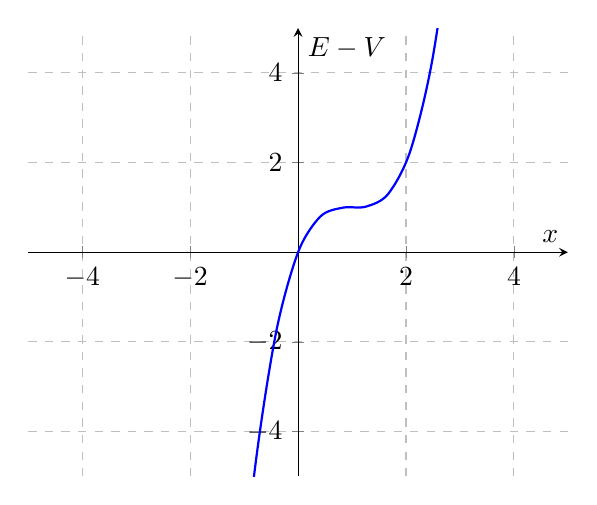
\begin{tikzpicture}
		\begin{axis}
			[
				axis lines=middle,
				xmin=-5,xmax=5,
				ymin=-5,ymax=5,
				xlabel=$x$,
				ylabel=$E-V$,
				ytick={-6,-4,-2,0,2,4,6},
				xtick={-6,-4,-2,0,2,4,6},
				yticklabels={$-6$,$-4$,$-2$,$0$,$2$,$4$},
				xmajorgrids=true,
				ymajorgrids=true,
				grid style=dashed,
				legend pos=north west
			]
			\addplot[smooth,thick,blue]{(x-1)^3+1};
		\end{axis}
	\end{tikzpicture}
\end{center}

我们假设能量与位势的差$E-V(x)$的是如上图的这样的一个形式,可以看到,这里会存在一个$E=V$的情况,这在我们之前的讨论当中是没有的,而我们的 connection formula 也是我为了将这个情况考虑进去。

考虑在原点处的修复波函数$\psi_p(x)$,于是,早这个点附近的势能$V(x)$可以进行一个泰勒展开来进行近似
\begin{align*}
	V(x)=E+V^\prime(x_0)(x-x_0)+\cdots
\end{align*}

带入到定态薛定谔方程当中,可以得到
\begin{align*}
	-\frac{\hbar^2}{2m}\frac{d^2}{dx^2}\psi_p+\left[E+V^\prime(x_0)(x-x_0)\right]\psi_p & =E\psi_p                                       \\
	\frac{d^2}{dx^2}\psi_p                                                              & = \frac{2m}{\hbar^2}V^\prime(x_0)(x-x_0)\psi_p
\end{align*}

化简一下,可以得到
\begin{align*}
	\frac{d^2}{dz^2}\psi_p & = z\psi_p
\end{align*}

其中$z\equiv \alpha(x-x_0),\alpha^3\equiv \dfrac{2m}{\hbar^2}V^\prime(x_0)$,同时这也是我们的艾里方程(Airy Equation).

同时这是一个二阶的微分方程,因此,这个方程的解将会是两个函数的线性叠加,写为
\begin{align*}
	\psi_p=aAi(\alpha x)+bBi(\alpha x)
\end{align*}

这个方程的解的形式为
\begin{align*}
	Ai(x) & =\frac{1}{\pi}\int_{0}^{+\infty}\cos(\frac{s^2}{3}+sz)ds                                  \\
	Bi(x) & =\frac{1}{\pi}\int_{0}^{+\infty}\left[e^{-\frac{s^2}{3}+sz}+\sin(\frac{s^2}{3}+sz)\right]
\end{align*}

通过以上的积分形式的解,我们可以得到其渐进形式
\begin{enumerate}
	\item[$z\geq  0$]
	      \begin{align*}
		      Ai(x) & \sim \frac{1}{2\sqrt{\pi}z^{1/4}}e^{-\frac{2}{3}z^{3/2}} \\
		      Bi(x) & \sim \frac{1}{\sqrt{\pi}z^{1/4}}e^{\frac{2}{3}z^{3/2}}
	      \end{align*}
	\item[$z\leq 0$]
	      \begin{align*}
		      Ai(x) & \sim \frac{1}{\sqrt{\pi}(-z)^{1/4}}\sin(\frac{2}{3}(-z)^{3/2}+\frac{\pi}{4}) \\
		      Bi(x) & \sim \frac{1}{\sqrt{\pi}(-z)^{1/4}}\cos(\frac{2}{3}(-z)^{3/2}+\frac{\pi}{4})
	      \end{align*}
\end{enumerate}













\end{document}
